\chapter{Literature Review}

%Similiar Studies Table Current Previous Research Conducted by other presented in table

%use triangle diagram Branching focusing graphical framework (Diagram tree) Research Gap 

\section{Review of Related Research}

To establish a baseline for the expected aerothermal outcomes, a review of key flight tests and numerical studies was conducted. Table \ref{tab:research_comparison} summarizes the landmarks in HIAD research that support the triangulation of results in this study.

\begin{longtable}{|p{3cm}|p{3.5cm}|p{4.5cm}|p{3cm}|}
\caption{Comparison of Landmark HIAD Aerothermal Research and Flight Tests} \label{tab:research_comparison} \\
\hline
\textbf{Research / Project} & \textbf{Key Geometry} & \textbf{Major Aerothermal Findings} & \textbf{Relevance to Outcome} \\ \hline
\endfirsthead
\multicolumn{4}{c}%
{{\bfseries \tablename\ \thetable{} -- continued from previous page}} \\
\hline
\textbf{Research / Project} & \textbf{Key Geometry} & \textbf{Major Aerothermal Findings} & \textbf{Relevance to Outcome} \\ \hline
\endhead
\hline \multicolumn{4}{|r|}{{Continued on next page}} \\ \hline
\endfoot
\hline
\endlastfoot

\textbf{NASA IRVE-3} (Lau et al., 2013) & 3-meter stacked-toroid HIAD. & Confirmed that "scalloping" (surface deflection) increases local heating compared to smooth surfaces. & Primary validation for the scalloped model. \\ \hline

\textbf{NASA LOFTID} (Cassell et al., 2022) & 6-meter large-scale HIAD with Gen-2 FTPS. & Demonstrated thermal survival during Earth reentry; identified transition onset on the flank. & Validates FTPS effectiveness at high enthalpy. \\ \hline

\textbf{Lichodziejewski et al. (2012)} & Deformed Outer Mold Line (OML) Analysis. & Proved that surface irregularities between tori significantly augment local heat flux. & Justifies the Config B (Smooth) comparison. \\ \hline

\textbf{HEART Project} (Cassell et al., 2014) & Optimized Nose-IAD Junction Geometry. & Found that the juncture between the nose and the IAD creates a secondary heat flux peak. & Predicts the location of local hot spots. \\ \hline

\textbf{Menter (1994)} & $k$-$\omega$ SST Turbulence Model. & Superior performance in predicting separation in adverse pressure gradients. & Supports model for valley recirculation. \\ \hline
\end{longtable}
\subsection{Triangulation of Expected Outcomes}
By synthesizing the findings of \textit{Lau et al. (2013)} and \textit{Lichodziejewski et al. (2012)}, it is hypothesized that the scalloped geometry in this study will generate localized heat flux peaks on the toroidal crests. 

Furthermore, the implementation of the \textit{SST $k-\omega$} turbulence model, as validated by \textit{Menter (1994)}, is expected to resolve the stable recirculation cells within the toroidal valleys. Finally, the use of a \textit{Thermally Perfect Gas} model reflects the high-enthalpy conditions observed in the \textit{LOFTID} mission, ensuring that the predicted shock physics align with real-gas observations rather than simplified ideal-gas assumptions.

This synthesis establishes the theoretical foundation for the numerical methodology described in \textbf{Chapter 3}.

\section{Fundamentals of Hypersonic Aerodynamics}

\par
Hypersonic flow is commonly as a rule of thumb being defined as the regime where the Mach number exceeds five ($M > 5$), though this threshold is more physical than mathematical. As a vehicle's velocity increases to several kilometers per second, the kinetic energy of the flow becomes so vast that its conversion into internal energy across shock waves and within viscous boundary layers fundamentally alters the gas behavior. 
\par
According to the classical frameworks established in hypersonic theory (Citation Needed), the flowfield is characterized by five distinct physical phenomena that distinguish it from supersonic flow:
\par
\begin{enumerate}
    \item \textbf{Thin Shock Layers:} At high Mach numbers, the shock wave lies very close to the body surface. For a blunt body, this results in a small stand-off distance, creating a high-pressure region between the shock and the vehicle.
    \item \textbf{Entropy Layers:} The strong curvature of the bow shock at the nose creates a region of high entropy gradient. As this layer flows downstream, it interacts with the boundary layer, complicating the pressure and heat transfer calculations.
    \item \textbf{Viscous Interaction:} The high temperature within the boundary layer reduces the local density, causing the boundary layer to grow rapidly ($\delta \propto M^2/\sqrt{Re}$). This thick layer displaces the outer inviscid flow, significantly altering the surface pressure distribution.
    \item \textbf{High-Temperature Effects:} The extreme kinetic energy is dissipated into thermal energy, triggering vibrational excitation, dissociation, and even ionization of the air molecules. This renders the calorically perfect gas assumption ($c_p = \text{const.}$) invalid.
    \item \textbf{Low-Density Effects:} At very high altitudes, the continuum assumption may begin to break down as the mean free path of the molecules becomes comparable to the vehicle's characteristic length.
\end{enumerate}
\par
For Inflatable Aerodynamic Decelerators (IADs), understanding these fundamentals is critical. The "scalloped" surface topology of stacked toroids interacts directly with the thin shock layer and viscous boundary layer, creating complex flow structures that do not exist on smooth-body vehicles.
\par


\subsection{Mach Number and the Hypersonic Regime (Ma $> 5$)}

The transition from supersonic to hypersonic flow is generally defined by the rule of thumb $Ma > 5$. Unlike the transition from subsonic to supersonic flow ($Ma = 1$), which is marked by a distinct physical discontinuity (the formation of shock waves), the boundary for hypersonic flow is not physically discrete. Instead, $Ma \approx 5$ represents the threshold where certain physical approximations used in linear supersonic theory lose accuracy, and high-temperature gas dynamics become significant \cite{AndersonHypersonic}.
\par

The distinguishing characteristic of this regime is the dominance of flow kinetic energy over internal energy. From the steady-flow energy equation, the total enthalpy $h_0$ is conserved across the shock wave:

\begin{equation}
    h_0 = h_{\infty} + \frac{1}{2}V_{\infty}^2 = h + \frac{1}{2}V^2
\end{equation}

Where $h$ is the static enthalpy and $V$ is the velocity. In the hypersonic regime, the freestream velocity $V_{\infty}$ is extremely high, meaning the kinetic energy term $\frac{1}{2}V_{\infty}^2$ is significantly larger than the static enthalpy $h_{\infty}$. As the flow decelerates to stagnation conditions ($V \approx 0$) at the nose of a blunt body (such as an IAD), this massive kinetic energy is converted almost entirely into internal energy (heat).
\par
This energy conversion scales with the square of the Mach number. For a calorically perfect gas, the ratio of stagnation temperature $T_0$ to freestream temperature $T_{\infty}$ is given by:

\begin{equation}
    \frac{T_0}{T_{\infty}} = 1 + \frac{\gamma - 1}{2} M_{\infty}^2
\end{equation}
\par
For a flight at $Ma = 5$ in standard air ($\gamma = 1.4$), the temperature rises by a factor of 6. At $Ma = 10$, it rises by a factor of 21. This exponential increase in temperature necessitates the coupling of thermodynamics with aerodynamics (aerothermodynamics), as the assumption of constant specific heats ($C_p$) is no longer valid due to vibrational excitation and dissociation of gas molecules.

\subsection{Shock Wave Formation and Properties}


In the hypersonic regime, the vehicle moves through the atmosphere significantly faster than the speed of sound, preventing pressure disturbances from propagating upstream. Consequently, these disturbances coalesce ahead of the vehicle to form a strong shock wave, a thin region of abrupt discontinuity in fluid properties \cite{AndersonHypersonic}.
\par
The thermodynamic changes across a normal shock wave are governed by the conservation of mass, momentum, and energy. These are collectively known as the Rankine-Hugoniot relations. For a calorically perfect gas, the ratio of downstream (post-shock, subscript 2) to upstream (pre-shock, subscript 1) properties is a function of the normal Mach number component ($M_n$):
\par
\begin{equation}
    \frac{p_2}{p_1} = 1 + \frac{2\gamma}{\gamma + 1} (M_n^2 - 1)
\end{equation}

\begin{equation}
    \frac{T_2}{T_1} = \left[1 + \frac{2\gamma}{\gamma + 1} (M_n^2 - 1)\right] \left[ \frac{2 + (\gamma - 1)M_n^2}{(\gamma + 1)M_n^2} \right]
\end{equation}

A critical distinction in hypersonic aerodynamics is the behavior of these ratios as the Mach number approaches infinity ($M \to \infty$). While pressure and temperature ratios increase indefinitely (leading to extreme aerodynamic heating), the density ratio approaches a finite limit:

\begin{equation}
    \lim_{M \to \infty} \frac{\rho_2}{\rho_1} = \frac{\gamma + 1}{\gamma - 1}
\end{equation}

For standard air ($\gamma = 1.4$), this limiting density ratio is $\rho_2/\rho_1 \approx 6$. This high compression means the mass flow is squeezed into a much smaller volume behind the shock compared to supersonic flow. This phenomenon is physically responsible for the formation of the Thin Shock Layer, where the shock wave "wraps" very closely around the body surface. This proximity is particularly important for the scalloped geometry of an IAD, as the shock structure may impinge upon the peaks of the toroidal rings, creating localized hotspots.

\begin{figure}[H]
    \centering
    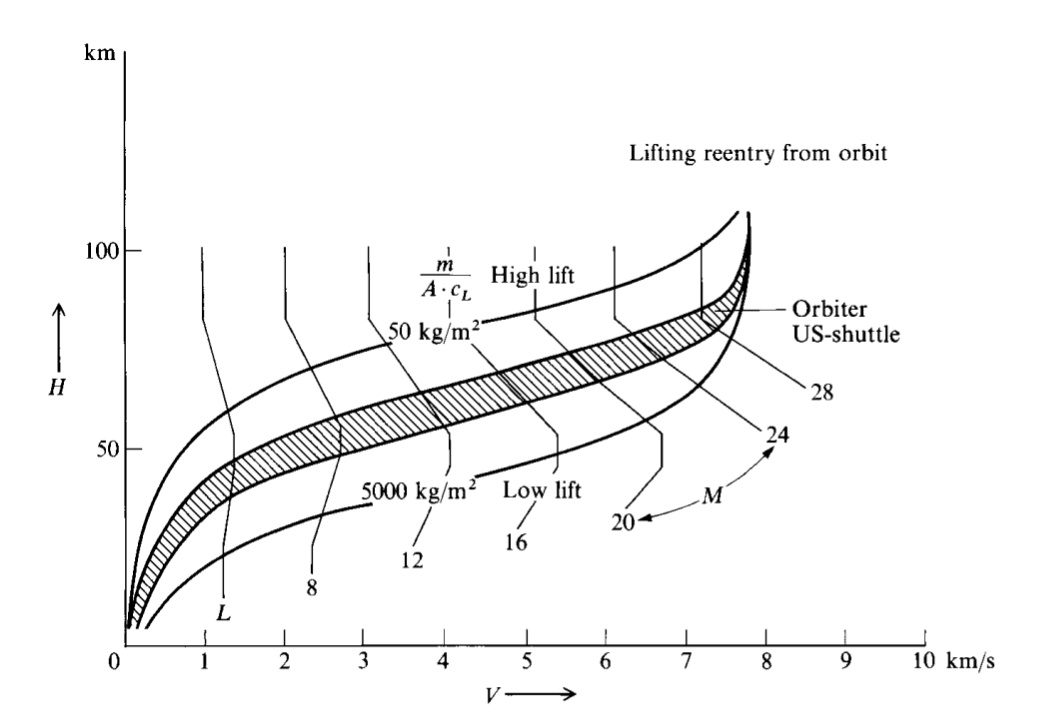
\includegraphics[width=0.8\textwidth]{figures/hypersonicMachandShockRelation.png}
    \caption{Figure for Shock Wave Formation and Properties Relation (Anderson, 2006)}
    \label{fig:shock_wave}
\end{figure}

\subsection{Invalidity of Subsonic/Supersonic Assumptions (Entropy layers, Viscous interaction)}
%\textit{Viscous Flow? Book theorem (Books Linkage)}

In lower-speed supersonic flows, aerodynamic analysis often decouples the inviscid outer flow from the viscous boundary layer. However, in the hypersonic regime ($Ma > 5$), this decoupling is often invalid due to two dominant phenomena: the Entropy Layer and Viscous Interaction \cite{AndersonHypersonic}.

\subsubsection*{The Entropy Layer}
For blunt bodies like an Inflatable Aerodynamic Decelerator (IAD), the bow shock is highly curved. The shock strength varies significantly from the normal shock at the stagnation streamline (strongest) to the oblique shock at the flanks (weaker). According to Crocco's Theorem, this curvature generates a strong gradient of entropy ($\Delta s$) across the streamlines behind the shock.
\par
This creates a layer of high-entropy, vortical flow—termed the "entropy layer"—that flows downstream and wets the vehicle surface. Unlike in supersonic flow, where this layer is negligible, in hypersonic flow, the entropy layer can be comparable in thickness to the boundary layer. This invalidates the standard boundary layer assumption that flow properties at the edge of the boundary layer are uniform/irrotational.
\par



\subsubsection*{Viscous Interaction}
A fundamental assumption in classical Prandtl boundary layer theory is that the pressure gradient is impressed upon the boundary layer by the outer inviscid flow (i.e., $\partial p / \partial y \approx 0$). In hypersonic flow, the massive kinetic energy converted to heat causes the temperature within the boundary layer to rise significantly. Since pressure is constant across the layer, the density decreases inversely with temperature ($\rho \propto 1/T$), causing the boundary layer displacement thickness ($\delta^*$) to grow rapidly:

\begin{equation}
    \delta^* \propto \frac{M_{\infty}^2}{\sqrt{Re_x}}
\end{equation}

This thick boundary layer acts as a new "effective" shape for the vehicle, displacing the outer inviscid flow and generating a completely different pressure distribution than what the geometric shape alone would suggest. This mutual dependence—where the boundary layer determines the pressure field, and the pressure field determines the boundary layer growth—is known as Hypersonic Viscous Interaction. For the scalloped geometry of the IAD, this interaction is critical in the valleys between toroids, where thick boundary layers may bridge the gaps and alter the effective aerodynamic shape.


\section{Aerothermodynamics of Re-entry Vehicles}
Aerothermodynamics represents the synthesis of high-speed aerodynamics and high-temperature thermodynamics, forming the cornerstone of atmospheric re-entry vehicle design. Unlike conventional aerodynamics, where the fluid is treated as a continuum with constant chemical properties, aerothermodynamics must account for the intense coupling between the flow field and the state of the gas \cite{AndersonHypersonic}.
\par
The fundamental challenge of re-entry is the dissipation of orbital energy. A spacecraft returning from Low Earth Orbit (LEO) possesses a velocity of approximately $7.8 \text{ km/s}$, while vehicles returning from lunar or Martian trajectories can exceed speeds of $11 \text{ km/s}$ \cite{AndersonHypersonic}. To reach the surface safely, this immense kinetic energy ($\frac{1}{2}mV^2$) and potential energy ($mgh$) must be converted into other forms—primarily thermal energy—without exceeding the structural limits of the vehicle or the physiological limits of the payload.
\par
This energy conversion occurs within the shock layer enveloping the vehicle. As the gas molecules are processed by the strong bow shock, their directed kinetic energy is randomized into internal energy, raising the static temperature of the shock layer to values often exceeding the temperature of the solar surface ($> 6000 \text{ K}$). At these extreme temperatures, the air acts as a chemically reacting plasma rather than a simple gas. The nitrogen and oxygen molecules dissociate ($N_2 \rightarrow 2N$, $O_2 \rightarrow 2O$) and, at higher speeds, ionize ($N \rightarrow N^+ + e^-$), significantly altering the thermodynamic and transport properties of the fluid (e.g., specific heat ratio $\gamma$, viscosity $\mu$, and thermal conductivity $k$).
\par
Consequently, the design of any re-entry system, including Hypersonic Inflatable Aerodynamic Decelerators (HIADs), is governed by the need to manage this heat load. The vehicle must be designed not only to withstand the integrated heat load (total heat soaked) but also the peak heat flux (maximum rate of heating) which occurs deep within the atmosphere where density increases. This creates a critical trade-off between aerodynamic deceleration (drag) and thermal management, dictating that the vehicle geometry must be optimized to maximize drag while minimizing the transfer of energy to the surface.

\begin{figure}[H]
    \centering
    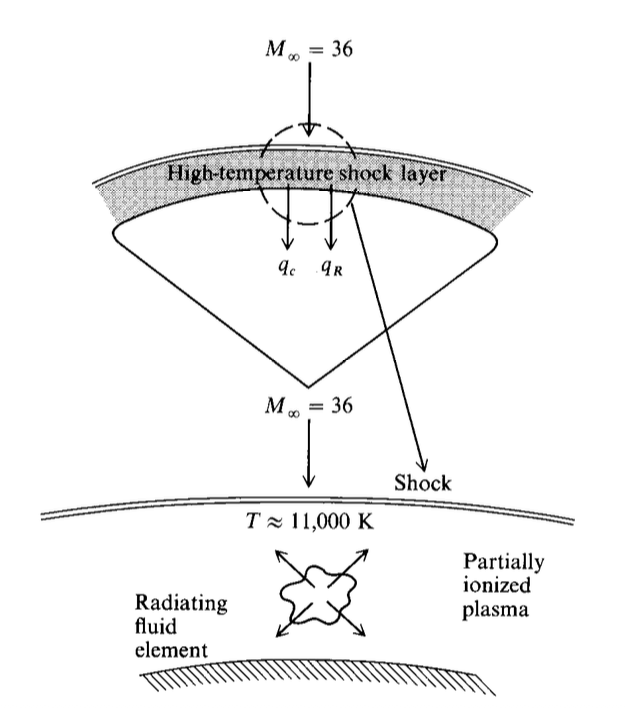
\includegraphics[width=0.8\textwidth]{figures/aerodynamicHighShockBody.png}
    \caption{Figure for Aerothermodynamics of Re-entry Vehicles.}
    \label{fig:aerothermodynamics}
\end{figure}

\subsection{Mechanisms of Aerodynamic Heating (Kinetic to Thermal energy conversion)}

The primary source of aerodynamic heating in hypersonic flight is the immense kinetic energy of the oncoming flow. As the vehicle arrests the flow, this directed kinetic energy is converted into internal thermal energy. This conversion occurs through two distinct physical mechanisms within the shock layer \cite{AndersonHypersonic}.



\subsubsection*{1. Shock Wave Compression}
As the supersonic freestream crosses the bow shock, the flow velocity decreases abruptly, and the pressure and density rise. This process is largely adiabatic but highly non-isentropic. The work done by pressure forces on the fluid elements compresses the gas, raising the static enthalpy ($h$) significantly. At the stagnation point, effectively all the freestream kinetic energy is converted to enthalpy, defined by the total enthalpy equation:

\begin{equation}
    h_0 = h_{\infty} + \frac{1}{2} V_{\infty}^2
\end{equation}

For a vehicle traveling at $Ma = 25$ (approximate re-entry speed), the total enthalpy is sufficient to dissociate nitrogen and oxygen, creating a chemically reacting plasma behind the shock.

\subsubsection*{2. Viscous Dissipation within the Boundary Layer}
While the shock wave processes the bulk flow, the interaction at the vehicle surface is governed by viscosity. Within the boundary layer, the fluid velocity must vanish at the wall ($u=0$) due to the no-slip condition. This deceleration is caused by shear stress ($\tau$) acting between adjacent fluid layers. The work done by these viscous forces against the velocity gradient generates heat, a phenomenon known as viscous dissipation.
\par
The local rate of heat transfer to the wall ($q_w$) is determined by the thermal gradient at the surface, governed by Fourier’s Law:

\begin{equation}
    q_w = -k_w \left( \frac{\partial T}{\partial y} \right)_{w}
\end{equation}

In hypersonic aerothermodynamics, it is convenient to express this heat flux in terms of the driving enthalpy potential. The heat flux is proportional to the difference between the recovery enthalpy ($h_{aw}$, the enthalpy of the gas if the wall were adiabatic) and the actual wall enthalpy ($h_w$):

\begin{equation}
    q_w = \rho_e u_e C_H (h_{aw} - h_w)
\end{equation}

Where $\rho_e$ and $u_e$ are the edge density and velocity, and $C_H$ is the Stanton number (heat transfer coefficient). This relationship highlights that heating is most severe where the boundary layer is thinnest (high gradients) and where the local flow energy is highest.


\subsection{Bow Shock Stand-off/detachment Distance}

\par
A defining characteristic of blunt-body aerodynamics in the hypersonic regime is the detachment of the shock wave from the vehicle's nose. Unlike sharp-edged bodies where the shock may be attached to the leading edge, the large radius of curvature of an Inflatable Aerodynamic Decelerator (IAD) forces the formation of a strong, curved normal shock ahead of the stagnation point. The physical separation between the shock wave and the body along the stagnation streamline is defined as the shock stand-off distance ($\Delta$).
\par
The magnitude of this stand-off distance is critically dependent on the density ratio across the shock. As derived in classical hypersonic theory \cite{AndersonHypersonic}, the conservation of mass requires that the mass flow entering the shock must exit through the annular area between the shock and the body. Because the post-shock density ($\rho_2$) is significantly higher than the freestream density ($\rho_{\infty}$), the required flow area is small, resulting in a thin shock layer.

For a spherical nose of radius $R$, the stand-off distance can be approximated by the correlation:

\begin{equation}
    \frac{\Delta}{R} \approx \frac{\rho_{\infty}}{\rho_2}
\end{equation}

More precise empirical correlations, such as Billig's approximation for a sphere, express this relationship as:

\begin{equation}
    \frac{\Delta}{R} = 0.143 \exp\left(\frac{3.24}{M_{\infty}^2}\right)
\end{equation}

This relationship has profound implications for IAD design. In hypersonic flow, where real gas effects (dissociation) can increase the density ratio $\rho_2/\rho_{\infty}$ well beyond the ideal gas limit of 6, the stand-off distance shrinks further. A smaller $\Delta$ increases the velocity gradients within the shock layer, which directly intensifies the convective heat transfer to the wall. For scalloped geometries, if the stand-off distance becomes comparable to the depth of the valleys between toroids, it can lead to complex shock-shock interactions or shock impingement on the structural surface.

\begin{figure}[H]
    \centering
    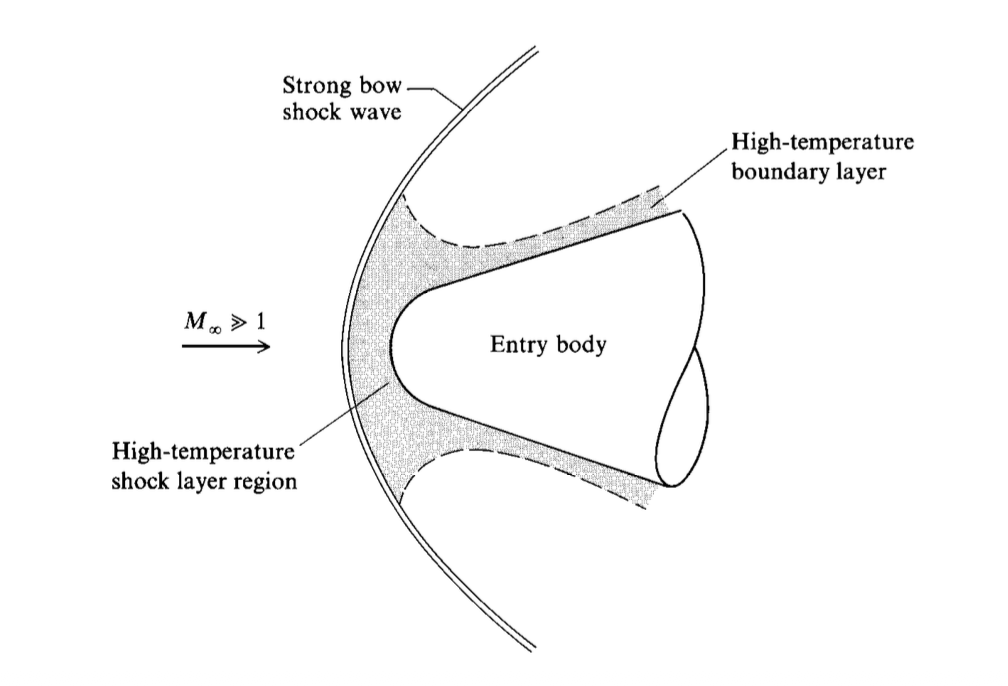
\includegraphics[width=0.8\textwidth]{figures/bowshock_figure1.png}
    \caption{Figure for Bow Shock Stand-off/detachment Distance. (Anderson, 2006)}
    \label{fig:bow_shock}
\end{figure}

\subsection{H. Julian Allen’s Blunt Body Theory }
%(Why drag and bowshock is good for heat management)
\par
In the early development of supersonic flight, the prevailing design philosophy favored sharp, slender noses to minimize aerodynamic drag. However, as speeds approached the hypersonic regime, H. Julian Allen and Alfred Eggers of NACA Ames Research Center revolutionized re-entry vehicle design with the Blunt Body Theory (1953) \cite{AndersonHypersonic}. This counter-intuitive theory established that while sharp bodies are efficient for supersonic cruise, they are catastrophic for hypersonic re-entry.
\par
The fundamental principle rests on the energy balance of the vehicle. The total kinetic energy lost by the re-entering body is dissipated into two sinks: heating the air (via shock compression) and heating the vehicle body (via viscous friction).

\begin{enumerate}
    \item \textbf{Sharp Body:} Creates a weak, attached shock wave. The wave drag is low, meaning the air is not heated significantly. Consequently, a large fraction of the kinetic energy is dissipated through skin friction directly on the surface, leading to extreme aerodynamic heating that can melt conventional materials.
    
    \item \textbf{Blunt Body:} Generates a strong, detached bow shock wave. This creates massive pressure drag (wave drag), which dissipates the majority of the kinetic energy into the airflow itself, creating a high-temperature wake behind the vehicle. Because the energy is dumped into the atmosphere rather than the structure, the heat load on the vehicle is drastically reduced.
\end{enumerate}

Allen mathematically demonstrated that the stagnation point heat flux ($q_s$) is inversely proportional to the square root of the nose radius ($R_n$), while the aerodynamic drag ($D$) is directly proportional to the projected area (and thus $R_n$):

\begin{equation}
    q_s \propto \frac{1}{\sqrt{R_n}} \quad \text{and} \quad D \propto R_n^2
\end{equation}

This relationship proves that increasing the bluntness of the vehicle not only increases drag (aiding deceleration) but simultaneously decreases the peak heat flux. This theorem is the theoretical foundation for Hypersonic Inflatable Aerodynamic Decelerators (HIADs), which utilize an extremely large effective radius to maximize drag and minimize localized heating, thereby enabling the entry of massive payloads into planetary atmospheres.

Here is example of the effect of the blunt body~\cite{aerospace9120800BluntBodyTheory}

\begin{figure}[H]
    \centering
    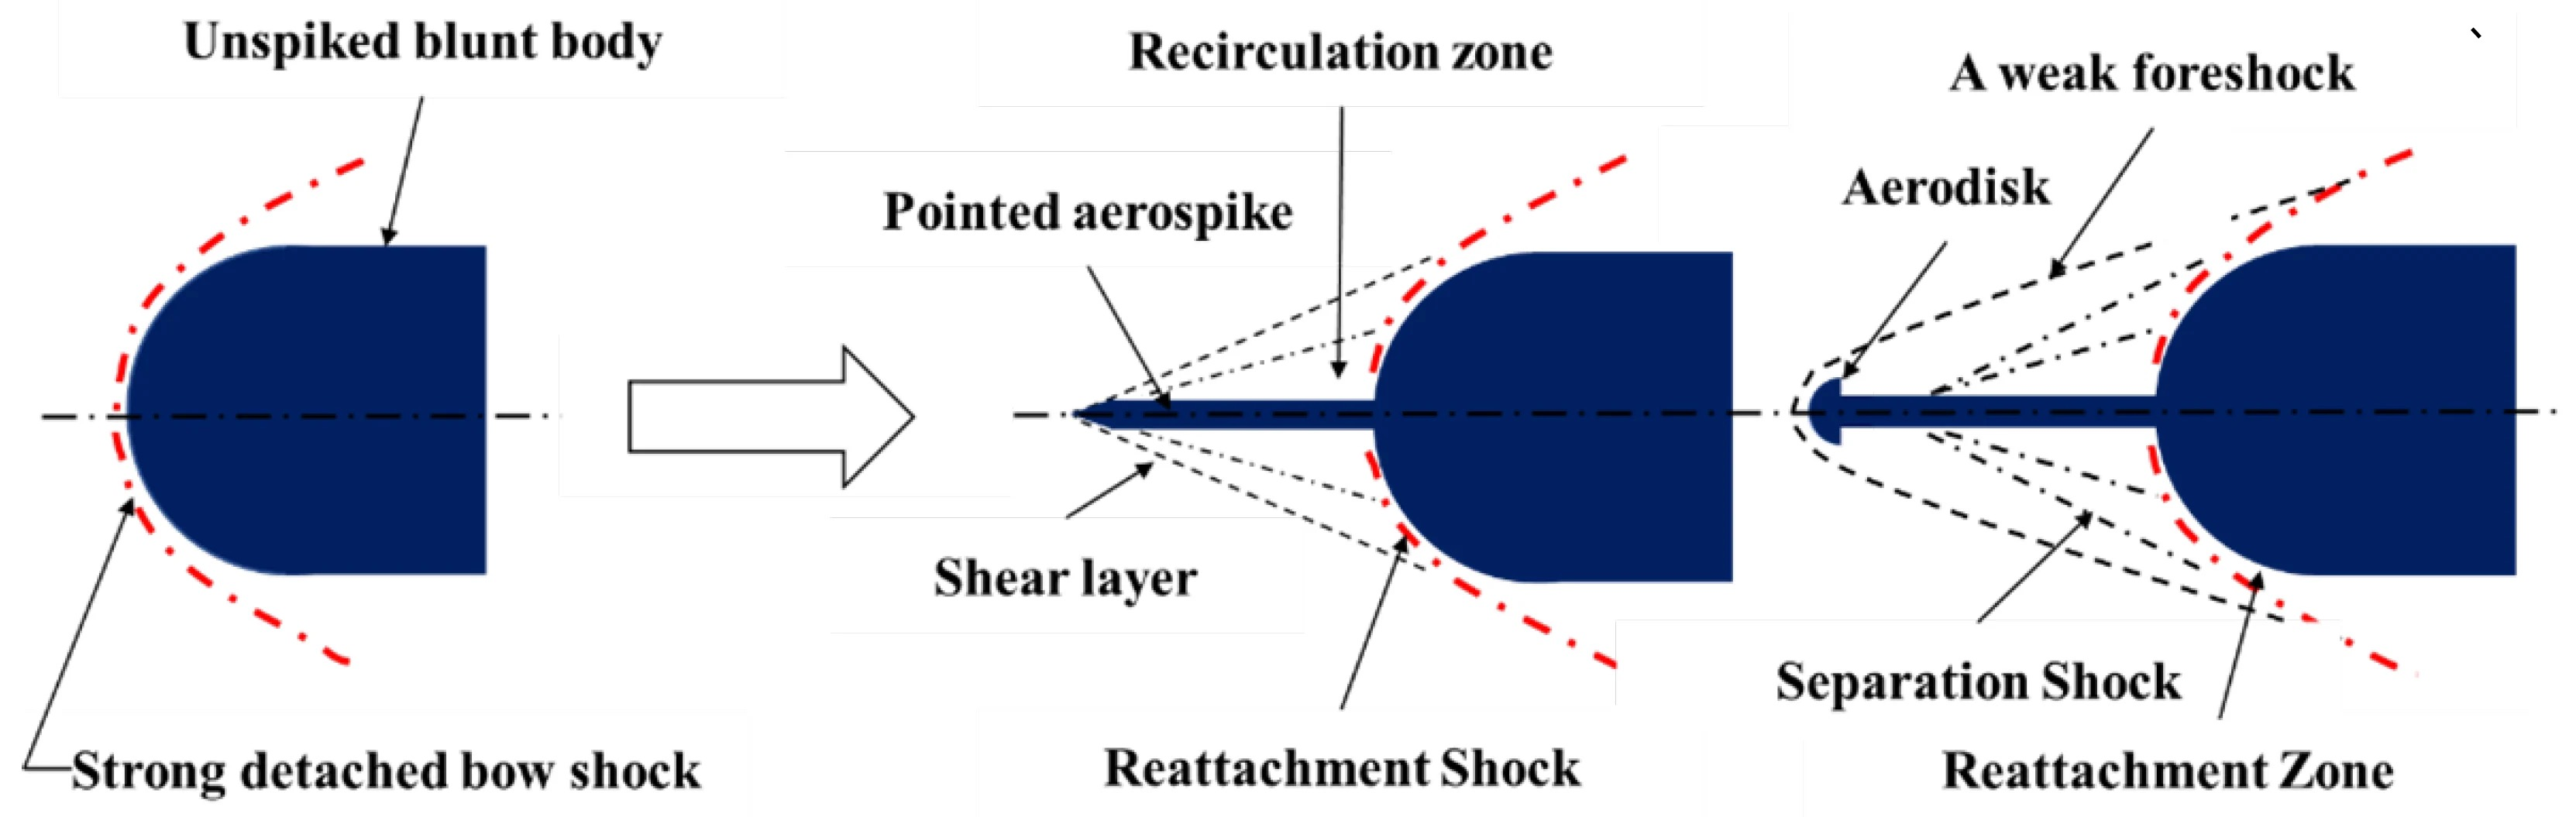
\includegraphics[width=0.8\textwidth]{figures/aerospace-09-00800-g001-bluntbodyTheory.png}
    \caption{Figure for H. Julian Allen’s Blunt Body Theory.}
    \label{fig:blunt_body_theory}
\end{figure}

\section{Thermal Protection Systems (TPS) Technology}
%\textit{Link with TPS AIAA or Nasa definition of TPS Paper technology about re-entry}

\par
The Thermal Protection System (TPS) is the single most critical subsystem for atmospheric entry vehicles, serving as the interface between the extreme aerothermal environment and the vehicle's structure. Its primary function is to maintain the inner structural bondline temperature below critical material limits (typically $< 175^\circ$C for aluminum or composite structures) while enduring surface temperatures that can exceed $2000^\circ$C \cite{TPS-stateofIndustryNASA}.
\par
Unlike other subsystems where redundancy can be engineered (e.g., avionics or propulsion), the TPS is often a "single point of failure" system; any breach or significant failure in the thermal barrier typically results in the loss of the vehicle \cite{AndersonHypersonic}.

TPS technologies are broadly categorized based on their mechanism of heat management:

\begin{enumerate}
    \item \textbf{Ablative TPS:} Designed for the most severe heating environments (e.g., steep re-entry or planetary probes). These materials manage heat loads through phase change (pyrolysis), chemically decomposing to create a char layer and releasing gases that thicken the boundary layer and block convective heating (blowing effect). Examples include PICA (Phenolic Impregnated Carbon Ablator) and Avcoat \cite{TPS-stateofIndustryNASA}.
    
    \item \textbf{Reusable TPS:} Designed for missions requiring multiple flights with minimal refurbishment (e.g., Space Shuttle, X-37B). These systems rely on high-emissivity coatings to re-radiate a significant portion of the incident heat flux back into the atmosphere ($q_{rad} \propto \epsilon T^4$) while acting as an insulator to retard heat conduction to the substructure. They do not undergo phase change and are typically limited to lower heat fluxes than ablators.
\end{enumerate}

Historically, TPS has been synonymous with "rigid" architectures—tiles, bricks, or heavy monolithic shields. However, the geometric limitations of rigid aeroshells (constrained by the launch vehicle fairing diameter) have necessitated the development of flexible, deployable architectures like HIADs to enable the landing of heavier payloads on Mars \cite{DiNonnoLOFTID}.

\begin{figure}[htbp]
    \centering
    
    \begin{minipage}[t]{0.45\textwidth}
        \centering
        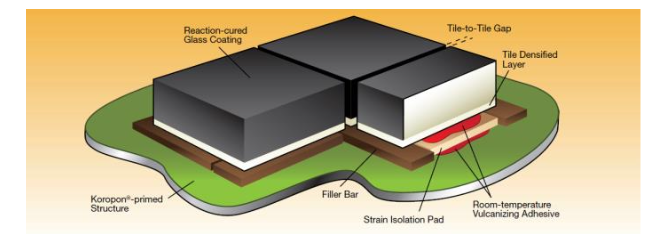
\includegraphics[width=0.9\linewidth]{figures/FigureTPSType0.png}
        \captionof{subfigure}{First Type Description}
        \label{fig:tps_type0}
    \end{minipage}
    \hfill
    \begin{minipage}[t]{0.45\textwidth}
        \centering
        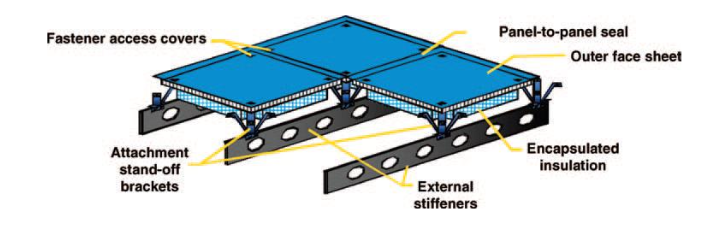
\includegraphics[width=0.9\linewidth]{figures/FigureTPSType1.png}
        \captionof{subfigure}{Second Type Description}
        \label{fig:tps_type1}
    \end{minipage}
    
    \vspace{0.5em}
    
    \begin{minipage}[t]{0.45\textwidth}
        \centering
        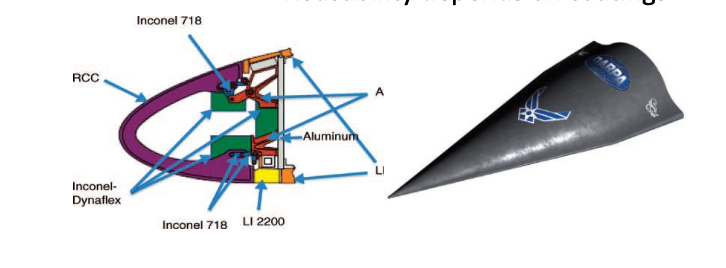
\includegraphics[width=0.9\linewidth]{figures/FigureTPSType2.png}
        \captionof{subfigure}{Third Type Description}
        \label{fig:tps_type2}
    \end{minipage}
    \hfill
    \begin{minipage}[t]{0.45\textwidth}
        \centering
        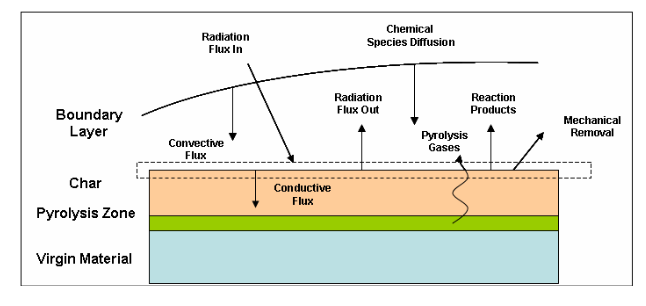
\includegraphics[width=0.9\linewidth]{figures/FigureTPSType3.png}
        \captionof{subfigure}{Fourth Type Description}
        \label{fig:tps_type3}
    \end{minipage}
    
    \caption{Classification of Thermal Protection Systems (TPS) Technology (Bouslog, 2023).}
    \label{fig:tps_technology_grid}
\end{figure}

\subsection{Conventional Rigid TPS (Ablative and Re-usable tiles)}
%\textit{Link with TPS AIAA or Nasa definition of TPS State of the Industry 3 types Jump from TPS-StateofInd-SAMPE-Final2 -> to 3 types example and it's effectiveness Paper technology about re-entry}
\par
For decades, the standard for atmospheric entry has been rigid TPS, which can be broadly categorized into three architectures based on their functionality and integration with the vehicle structure \cite{TPS-stateofIndustryNASA}.

\subsubsection*{1. Ablative TPS}
Ablative systems are the workhorses of high-energy planetary entry (e.g., Apollo, Mars Science Laboratory). They function by sacrificing material to manage the extreme heat load. As the surface temperature rises, the polymer matrix undergoes pyrolysis—an endothermic chemical decomposition that absorbs energy. This process generates a porous char layer that radiates heat away ($\epsilon \approx 0.9$) and releases pyrolysis gases (blowing) that thicken the boundary layer, physically pushing the high-temperature shock layer away from the wall.
\begin{itemize}
    \item \textbf{Example:} PICA (Phenolic Impregnated Carbon Ablator) used on SpaceX Dragon and NASA's Stardust mission.
    \item \textbf{Limitation:} They are typically single-use and heavy, and their rigid nature limits the vehicle diameter to the size of the launch fairing.
\end{itemize}



\subsubsection*{2. Reusable Surface Insulation (RSI)}
Made famous by the Space Shuttle Orbiter, these systems consist of lightweight ceramic tiles or blankets (e.g., LI-900 silica tiles) designed to survive thousands of degrees without ablating. They rely on extremely low thermal conductivity to insulate the aluminum airframe and high surface emissivity to re-radiate up to 90\% of the incident heat back into space.
\begin{itemize}
    \item \textbf{Example:} HRSI (High-Temperature Reusable Surface Insulation) black tiles.
    \item \textbf{Limitation:} They are extremely fragile, labor-intensive to install/maintain, and cannot withstand the heat fluxes associated with high-speed lunar or Martian return trajectories.
\end{itemize}

\subsubsection*{3. Hot Structures}
In this architecture, the primary load-bearing structure itself serves as the thermal protection. Materials like Carbon-Carbon (C-C) or ceramic matrix composites (CMCs) are used for nose caps and wing leading edges where temperatures are highest ($> 1500^\circ$C).
\begin{itemize}
    \item \textbf{Example:} The Reinforced Carbon-Carbon (RCC) nose cap of the Space Shuttle.
\end{itemize}

While effective, these rigid technologies fundamentally constrain the ballistic coefficient ($m/C_d A$) of the vehicle. To land heavier payloads on Mars, the drag area ($A$) must be increased beyond the limits of rigid fairings, necessitating the shift toward flexible, deployable architectures \cite{DiNonnoLOFTID}.

\begin{figure}[H]
    \centering
    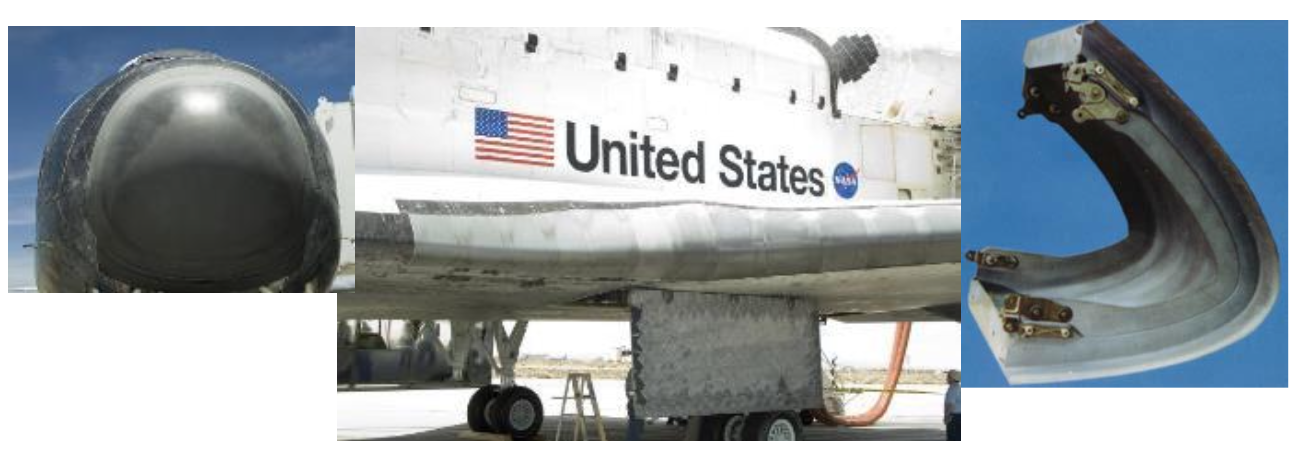
\includegraphics[width=0.8\textwidth]{figures/ReinforcedNoseStaticTPS.png}
    \caption{Figure for Conventional Rigid TPS.}
    \label{fig:rigid_tps}
\end{figure}

\subsection{Hypersonic Inflatable Aerodynamic Decelerators (HIAD/LOFTID)}
%\textit{Link with HIAD LOFTID}
%\par
To overcome the diameter constraints imposed by launch vehicle fairings, NASA and commercial partners have developed Hypersonic Inflatable Aerodynamic Decelerators (HIADs). A HIAD is a deployable aeroshell consisting of an inflatable structural backbone covered by a Flexible Thermal Protection System (FTPS) \cite{DiNonnoLOFTID}.



\subsubsection*{Structural Architecture}
The structural core of a HIAD typically comprises a stack of pressurized toroidal tubes (tori) made of high-strength braided synthetic fibers (e.g., Kevlar or Vectran). These toroids are strapped together to form a blunt cone shape. Unlike a smooth rigid shell, this construction inherently creates a "scalloped" or wavy surface topology, where the radius of each toroid creates a series of peaks (crests) and valleys. This specific geometry is the focus of the aerodynamic analysis in this thesis, as it introduces complex flow interactions not present on smooth bodies.

\subsubsection*{The LOFTID Mission}
The technology reached a major milestone with the Low-Earth Orbit Flight Test of an Inflatable Decelerator (LOFTID), successfully conducted in August 2015. The LOFTID vehicle, a 6-meter diameter aeroshell, demonstrated the ability of an inflatable structure to survive the hypersonic heat pulse of re-entry ($> 1400^\circ$C) and successfully decelerate a payload from orbital velocity \cite{DiNonnoLOFTID}.

LOFTID validated two critical advantages of this technology:
\begin{itemize}
    \item \textbf{Packaging Efficiency:} The entire 6-meter aeroshell was packed into a space significantly smaller than its deployed diameter, allowing it to fit within a standard Atlas V payload fairing.
    \item \textbf{Ballistic Coefficient Management:} By deploying a large drag area ($A$), the ballistic coefficient ($\beta = m/C_d A$) is drastically reduced. This allows deceleration to occur higher in the atmosphere where density (and thus heating) is lower, a capability essential for landing heavy payloads on the high-elevation surface of Mars.
\end{itemize}


\begin{figure}[H]
    \centering
    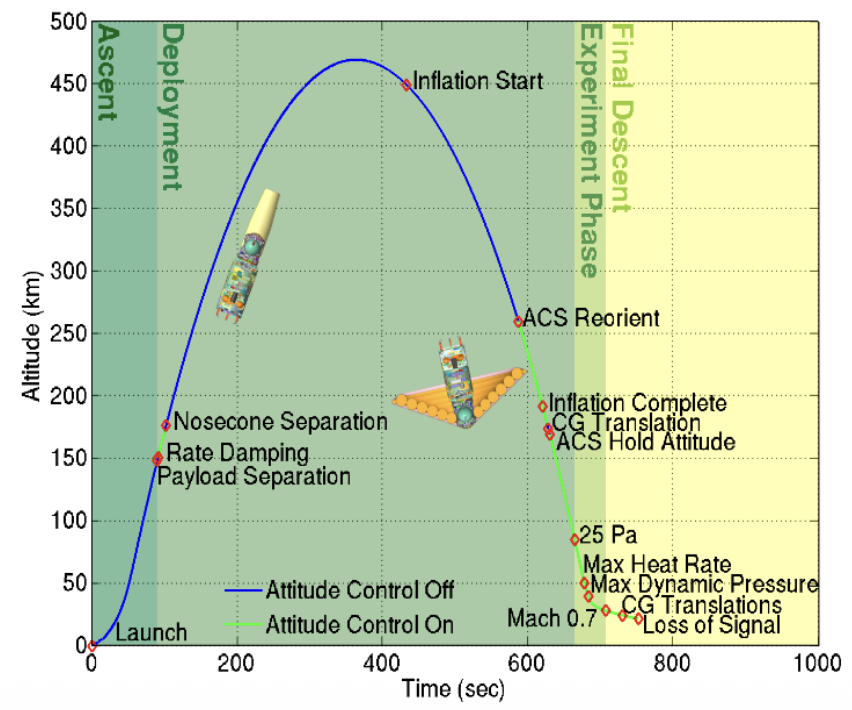
\includegraphics[width=0.8\textwidth]{figures/LOFTID_mission_trajectory.png}
    \caption{LOFTID Mission Trajectory}
    \label{fig:LoftidMission}
\end{figure}


\begin{figure}[H]
    \centering
    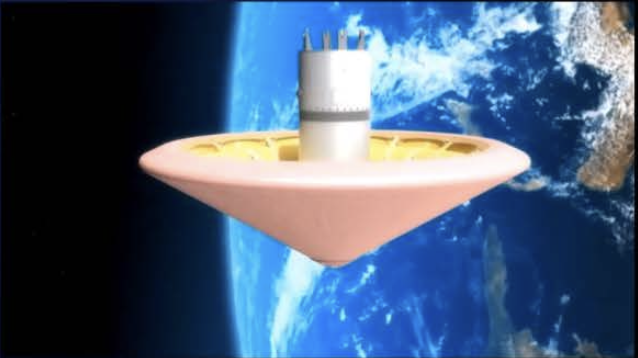
\includegraphics[width=0.8\textwidth]{figures/HIADsDeployed.png}
    \caption{Figure for HIAD/LOFTID.}
    \label{fig:hiad_loftid}
\end{figure}

\subsection{Comparison of Rigid vs. Flexible Structures}
\textit{Link with TPS AIAA or Nasa definition of TPS State of the Industry 3 types Jump from TPS-StateofInd-SAMPE-Final2 -> to 3 types example and it's effectiveness Paper technology about re-entry}
\par
The transition from conventional rigid aeroshells to flexible inflatable decelerators represents a paradigm shift in entry system design. While rigid TPS relies on a fixed outer mold line (OML) to maintain aerodynamic stability, flexible structures introduce a dynamic coupling between the aerodynamic loads and the structural response \cite{DiNonnoLOFTID}.



The primary distinction lies in the management of the Ballistic Coefficient ($\beta$). Rigid vehicles are volume-constrained by the launch shroud, forcing a high $\beta$ which results in peak heating occurring deep in the atmosphere. In contrast, HIADs decouple the entry diameter from the launch diameter, allowing for a much lower $\beta$. This enables deceleration at higher altitudes, significantly reducing the heat flux requirements.

However, the flexibility of the IAD introduces complexities absent in rigid designs. The "scalloped" surface of the stacked toroids creates a rough aerodynamic profile that can augment local heating, and the structural deformation under drag loads can alter the vehicle's stability characteristics.

A comparative summary of the two architectures is presented in Table \ref{tab:tps_comparison}.

\begin{table}[H]
    \centering
    \caption{Comparison of Conventional Rigid TPS and Hypersonic Inflatable Aerodynamic Decelerators (HIAD).}
    \label{tab:tps_comparison}
    \begin{tabularx}{\textwidth}{|l|X|X|}
        \hline
        \rowcolor{gray!20} \textbf{Parameter} & \textbf{Rigid Aeroshell (Capsule)} & \textbf{Flexible/Inflatable (HIAD)} \\ \hline
        \textbf{Launch Constraint} & Diameter limited by launch vehicle fairing (e.g., 4-5 m). & Packable; deployed diameter can exceed fairing size (e.g., $>$ 10 m). \\ \hline
        \textbf{Surface Geometry} & Smooth, continuous Outer Mold Line (OML). & Scalloped/Wavy surface due to stacked toroids. \\ \hline
        \textbf{Aerodynamic Drag} & Lower drag area ($A$); higher Ballistic Coefficient. & Massive drag area ($A$); lower Ballistic Coefficient. \\ \hline
        \textbf{Thermal Management} & Ablation (phase change) or Re-radiation (tiles). & Flexible insulation layers (FTPS) with gas barriers. \\ \hline
        \textbf{Structural Response} & Static; shape remains constant under load. & Dynamic; structure deforms/deflects under aerodynamic load (FSI). \\ \hline %FSI (This is not flexible perhaps other part)
        \textbf{Mission Profile} & Lunar return, LEO return, small Mars probes. & Heavy-mass Mars landers, engine recovery. \\ \hline
    \end{tabularx}
\end{table}
\section{Impact of Surface Geometry on Flow Physics}
%\textit{Topology of Aerodynamics Scalloped physics (Sidenote: Can we compare this with a golf ball theorem then we can derived it from there)}
%\par
The aerodynamic design of conventional re-entry vehicles typically prioritizes smooth, continuous Outer Mold Lines (OML) to ensure predictable boundary layer development and uniform heat distribution. However, the structural architecture of a HIAD, composed of stacked pressurized toroids, inherently introduces a "scalloped" or wavy surface topology.
\par
This deviation from a smooth surface fundamentally alters the flow physics. To understand these effects, it is useful to draw a comparison with the classic "golf ball" phenomenon in fluid mechanics. In the subsonic regime, the dimples on a golf ball act as surface roughness elements that trip the laminar boundary layer into turbulence. This energized turbulent boundary layer is better able to resist adverse pressure gradients, thereby delaying flow separation and significantly reducing pressure drag (form drag).

However, in the hypersonic regime of an IAD, the physics of surface waviness serve a completely different dynamic:
\begin{itemize}
    \item \textbf{Scale:} The "valleys" between toroids are macro-scale features, not micro-roughness.
    \item \textbf{Objective:} Unlike a golf ball where the goal is drag \textit{reduction}, the goal of an IAD is drag \textit{maximization}.
    \item \textbf{Thermal Consequence:} While turbulence on a golf ball is purely beneficial for aerodynamics, turbulence on a hypersonic vehicle creates a severe penalty: it can increase surface heat flux by a factor of 3 to 5 compared to laminar flow \cite{AndersonHypersonic}.
\end{itemize}

Therefore, the study of the scalloped topology is not focused on drag reduction, but rather on the Aerothermal specifically, how the peaks (crests) and valleys of the toroids modify the shock structure and local heating rates. ~\cite{white2006viscous}

\begin{figure}[H]
    \centering
    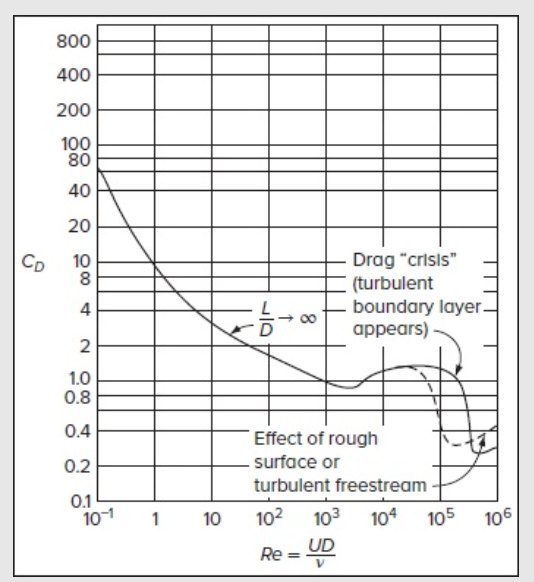
\includegraphics[width=0.8\textwidth]{figures/GolfBallImpactReImpact.png}
    \caption{Figure for Impact of Surface Topology on Re Number.}
    \label{fig:surface_topology}
\end{figure}

\subsection{Flow over Wavy and Scalloped Walls}
%\textit{Topology of Aerodynamics Scalloped physics (Sidenote: Can we compare this with a golf ball theorem then we can derived it from there)}
\par
The surface of an IAD can be mathematically approximated as a periodic wavy wall or a series of cavity steps. As the hypersonic flow traverses this undulating surface, it encounters alternating regions of favorable and adverse pressure gradients, a phenomenon fundamentally distinct from flow over a flat plate.
The physics can be derived by analyzing the momentum equation along the streamline. As the fluid moves over a convex crest (the peak of a toroid), the flow area effectively constricts, causing the flow to accelerate. According to Bernoulli's principle (and its compressible counterpart), this acceleration results in a local decrease in static pressure:

\begin{equation}
    \frac{dp}{dx} < 0 \quad (\text{Favorable Gradient - Crest})
\end{equation}

Conversely, as the flow descends into the concave valley between toroids, the flow area expands and the fluid decelerates. This deceleration generates a localized high-pressure region:

\begin{equation}
    \frac{dp}{dx} > 0 \quad (\text{Adverse Gradient - Valley})
\end{equation}

This creates a recurring cycle of expansion and compression.
\begin{itemize}
    \item \textbf{Over the Crests:} The flow undergoes an expansion fan process, turning away from the shock. The boundary layer thins, and the shear stress ($\tau_w$) increases, leading to peak heating.
    \item \textbf{In the Valleys:} The adverse pressure gradient forces the boundary layer to thicken. If the gradient is strong enough (i.e., the valley is deep), the momentum of the fluid near the wall is insufficient to overcome the pressure rise. This causes the flow to detach, creating a separation bubble or recirculation zone similar to the flow inside a golf ball dimple, but on a macroscopic scale.
\end{itemize}

This separation is critical for thermal management. In an ideal scenario, a stable recirculation vortex forms in the valley, allowing the high-energy outer flow to "skim" over the top of the gap. This effectively shields the valley floor from the extreme heat of the freestream, a mechanism analogous to the "trapped vortex" combustor concepts in propulsion.


\subsection{Shock-Boundary Layer Interaction (SBLI) on Rough Surfaces}
%\textit{FSI Book reference is unknown, require questioning.}
On a smooth hypersonic vehicle, the boundary layer typically grows monotonically from the stagnation point. However, the scalloped surface of an IAD acts as a "rough" wall with large-scale asperities, forcing a complex coupling between the inviscid shock system and the viscous boundary layer, known as Shock-Wave/Boundary-Layer Interaction (SBLI).
\par
This interaction is driven by the compression waves generated at the windward face of each toroid. As the flow exits a valley and encounters the upstream face of the next toroid, the geometry forces the flow to turn into itself (concave turning). In supersonic flow, this turning generates a compression wave or an oblique shock.
\par
This localized shock wave penetrates the boundary layer, imposing a strong adverse pressure gradient ($\frac{dp}{dx} > 0$).
\begin{itemize}
    \item \textbf{Separation:} If the shock is strong enough, the adverse pressure gradient can propagate upstream through the subsonic portion of the boundary layer, causing the flow to separate before it even reaches the valley floor.
    \item \textbf{Reattachment Shock:} When the separated shear layer reattaches to the crest of the next toroid, the flow is forced to align with the wall again. This re-alignment generates a Reattachment Shock.
\end{itemize}

The intersection of this reattachment shock with the boundary layer is a critical design concern. At the point of reattachment, the boundary layer is extremely thin (high velocity gradient), and the impinging shock further compresses the fluid. This combination results in a localized spike in both pressure and heat flux, which can be significantly higher than the stagnation point heating values predicted for a smooth body \cite{AndersonHypersonic}.\cite{aerospace10080729SWBLISBLI}

\begin{figure}[H]
    \centering
    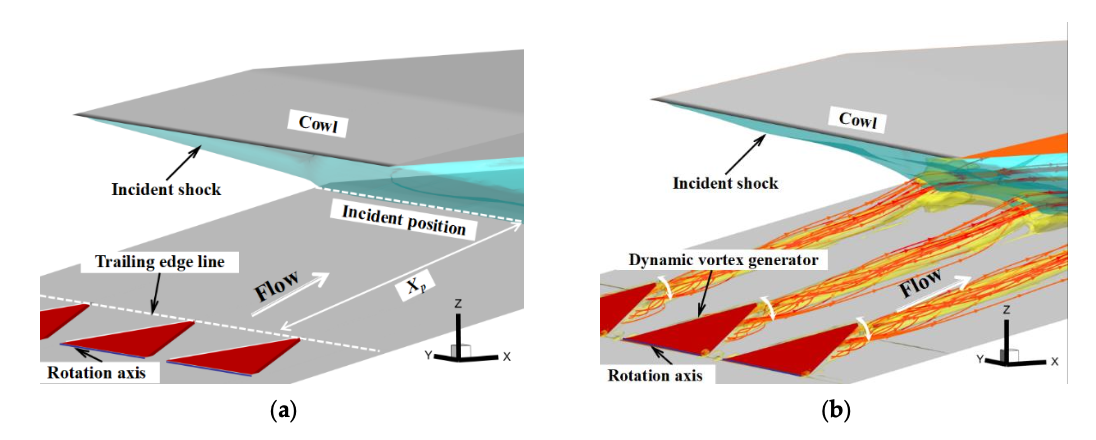
\includegraphics[width=0.8\textwidth]{figures/swblishockinteract.png}
    \caption{Figure for Shock-Boundary Layer Interaction (SBLI) or (SWBLI) on Rough Surfaces.}
    \label{fig:sbli}
\end{figure}

\subsection{Recirculation Zones and Stagnation in Surface Valleys}
%\textit{Recirculation Book reference is unknown, require questioning.}
\subsubsection*{The Shear Layer and Vortex Formation}
This free shear layer acts as a fluid dynamic boundary.
\begin{itemize}
    \item \textbf{Shear Layer:} A thin region of high vorticity where the velocity transitions from the freestream speed ($u_e$) to the near-zero velocity of the cavity.
    \item \textbf{Primary Vortex:} Driven by the shear stress at the interface, the fluid mass trapped within the valley is set into rotational motion, creating a large, stable recirculation structure known as the primary vortex.
\end{itemize}

\subsubsection*{Stagnation and Heat Alleviation}
Ideally, this recirculation zone creates a "dead air" region. The fluid deep within the valley has very low kinetic energy compared to the freestream. Consequently, the convective heat transfer is significantly reduced because the shear layer shields the valley floor from the high-enthalpy gradients of the shock layer.

However, the stability of this zone is dependent on the geometry of the valley, specifically the length-to-depth ratio ($L/D$).
\begin{itemize}
    \item \textbf{Open Cavity ($L/D < 10$):} The shear layer bridges the entire gap and reattaches at the downstream corner (next crest). This is the desired state for an IAD, as it maintains low heating in the valley.
    \item \textbf{Closed Cavity ($L/D > 10$):} If the valley is too wide or shallow, the shear layer may curve inward and impinges on the valley floor. This stagnation of the shear layer on the bottom surface would result in a local "hot spot" of high pressure and heating, negating the thermal benefits of the scalloped design.
\end{itemize}

This is as for example what is recirculation effect on an structure~\cite{RecirculationCaseWindDrivenCoastal}

\begin{figure}[H]
    \centering
    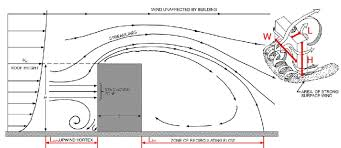
\includegraphics[width=0.8\textwidth]{figures/RecirculationExample.jpeg}
    \caption{Figure for Recirculation Zones and Stagnation Valleys Example on different scenarios.}
    \label{fig:recirculation_zones}
\end{figure}

\subsection{Localized Peak Heating Effects}
%\textit{Link with Hypersonic and High Temperature Gas Book (3 Book Linkage) (derivation on the mathematics of stagnation point of Mach number)}
While the recirculation zones in the valleys may alleviate thermal loads, the protruding crests of the toroidal rings experience the opposite effect: severe localized heating. This phenomenon is governed by the mathematics of stagnation point flow, where the local geometry creates conditions significantly more severe than the average heating over the vehicle.

\subsubsection*{The Stagnation Temperature (Energy Potential)}
The potential for heat transfer is driven by the total energy of the flow. As the fluid decelerates to zero velocity at a stagnation point (such as the windward face of a toroid), its kinetic energy is converted to enthalpy. For a calorically perfect gas, the stagnation temperature $T_0$ is a function of the freestream Mach number $M_{\infty}$ \cite{AndersonHypersonic}:

\begin{equation}
    \frac{T_0}{T_{\infty}} = 1 + \frac{\gamma - 1}{2} M_{\infty}^2
\end{equation}

For a hypersonic flow of $Ma=5$ (where $\gamma=1.4$), the stagnation temperature is six times the freestream temperature. This $T_0$ represents the driving potential for heat transfer.

\subsubsection*{The Geometric Scaling (Heat Flux Rate)}
While $T_0$ determines the \textit{temperature} limit, the \textit{rate} at which heat enters the structure ($q_s$) is determined by the velocity gradient at the wall. According to the classical Fay-Riddell correlation, the stagnation point heat flux scales inversely with the square root of the nose radius ($R_n$):

\begin{equation}
    q_s \approx 0.76 \cdot Pr^{-0.6} \cdot (h_{0} - h_w) \cdot \sqrt{\rho_e \mu_e} \cdot \sqrt{\left( \frac{du_e}{dx} \right)_s}
\end{equation}

The velocity gradient term $\left( \frac{du_e}{dx} \right)_s$ for a blunt body is geometrically dependent on the radius of curvature $R$:

\begin{equation}
    \left( \frac{du_e}{dx} \right)_s \approx \frac{V_{\infty}}{R} \sqrt{\frac{2 \rho_{\infty}}{\rho_{0}}}
\end{equation}

Substituting this back into the heat flux equation yields the critical proportionality:

\begin{equation}
    q_s \propto \sqrt{\frac{1}{R}}
\end{equation}

This derivation highlights the critical vulnerability of scalloped IAD geometries. While the \textit{overall} effective radius of the vehicle is large (low global heating), the \textit{local} radius of an individual toroid tube ($R_{tube}$) is small. Consequently, the crest of each toroid acts as a local stagnation point with a small radius, leading to "peak heating" spikes that can be significantly higher than the heating on a smooth sphere-cone of the same size.

It is demonstrated on the analogue of the localized heating \cite{daub2022experimentsElasticLocalizedHeating}

\begin{figure}[H]
    \centering
    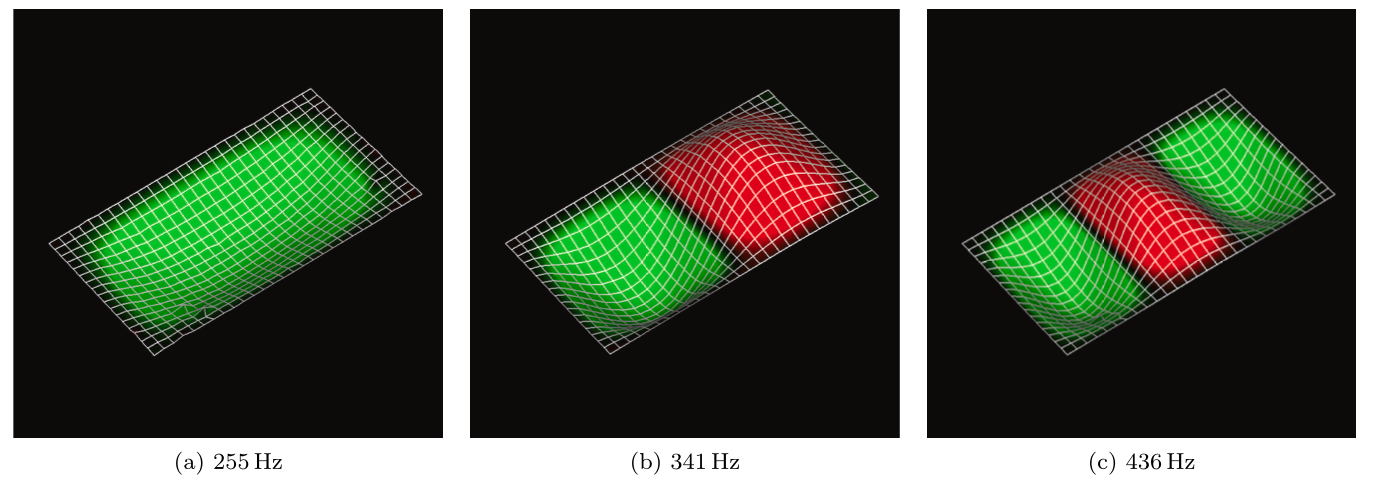
\includegraphics[width=0.8\textwidth]{figures/LocalizedHeatinginAmplify.png}
    \caption{Figure for Localized Peak Heating Effects in Amplification but through Osicaltion.}
    \label{fig:peak_heating}
\end{figure}

\section{Theoretical Framework of CFD}
%\textit{CFD Book () Linkage}
%\par
Computational Fluid Dynamics (CFD) serves as the third pillar of fluid dynamics research, complementing theoretical analysis and experimental testing. It involves the systematic application of numerical methods to solve the governing equations of fluid motion, transforming the continuous mathematical models into discrete algebraic equations that can be solved computationally \cite{versteeg2007cfd}.
\par
For hypersonic research, where flight tests are prohibitively expensive and ground-based facilities (such as wind tunnels) often suffer from scaling limitations or wall interference, CFD provides a critical capability to resolve complex flow physics. By discretizing the spatial domain into a grid, CFD allows for the detailed interrogation of flow properties—such as shock structures and thermal gradients—that are often difficult to measure experimentally.
\par
The theoretical foundation of this analysis rests upon the Continuum Hypothesis. This assumption treats the fluid not as a collection of discrete molecules, but as a continuous substance where macroscopic properties (density, pressure, velocity, and temperature) are well-defined at every point in space and time. Based on this hypothesis, the flow physics are governed by three fundamental conservation laws:
\begin{itemize}
    \item Conservation of Mass (Continuity)
    \item Conservation of Momentum (Newton's Second Law)
    \item Conservation of Energy (First Law of Thermodynamics)
\end{itemize}

\subsection{The Navier-Stokes Equations (Conservation of Momentum)}

The conservation of momentum is based on Newton's Second Law of Motion, which states that the rate of change of momentum of a fluid particle is equal to the sum of the forces acting on it.
\par
For an infinitesimal fluid element of volume $dV = dx dy dz$, the forces are categorized into two types:
\begin{itemize}
    \item \textbf{Surface Forces:} Forces acting on the boundaries of the element, including pressure ($p$) and viscous stresses ($\tau$).
    \item \textbf{Body Forces:} Forces acting on the entire mass of the element (e.g., gravity), denoted by the source term $S_M$.
\end{itemize}

\subsubsection*{1. The Momentum Balance}
Consider the $x$-component of momentum. The net force due to surface stresses in the $x$-direction is the sum of the gradients of the normal stress ($\sigma_{xx}$) and shear stresses ($\tau_{yx}, \tau_{zx}$). The general differential form for the conservation of momentum in the $i$-direction (where $i=x,y,z$) is given by \cite{versteeg2007cfd}:

\begin{equation}
    \frac{\partial (\rho u_i)}{\partial t} + \nabla \cdot (\rho u_i \mathbf{u}) = \nabla \cdot \sigma_{ij} + S_{M,i}
\end{equation}

Where the left-hand side represents the rate of change of momentum (transient + convective), and the right-hand side represents the forces. The stress tensor $\sigma_{ij}$ includes the thermodynamic pressure and the viscous stress tensor $\tau_{ij}$:

\begin{equation}
    \sigma_{ij} = -p \delta_{ij} + \tau_{ij}
\end{equation}

\subsubsection*{2. Constitutive Relations (Newtonian Fluid)}
To close the system of equations, the viscous stresses must be related to the velocity gradients (strain rates). For a \textbf{Newtonian fluid}, the viscous stress is proportional to the rate of deformation. This relationship is defined by:

\begin{equation}
    \tau_{ij} = \mu \left( \frac{\partial u_i}{\partial x_j} + \frac{\partial u_j}{\partial x_i} \right) + \lambda \delta_{ij} (\nabla \cdot \mathbf{u})
\end{equation}

Here, $\mu$ is the dynamic viscosity, and $\lambda$ is the second coefficient of viscosity. Following Stokes' hypothesis for monoatomic gases, we assume $\lambda = -\frac{2}{3}\mu$. This leads to the final form of the viscous stress tensor for a compressible flow:

\begin{equation}
    \tau_{ij} = \mu \left[ \left( \frac{\partial u_i}{\partial x_j} + \frac{\partial u_j}{\partial x_i} \right) - \frac{2}{3} (\nabla \cdot \mathbf{u}) \delta_{ij} \right]
\end{equation}

\subsubsection*{3. The Complete Navier-Stokes Equation}
Substituting the constitutive relation back into the momentum equation yields the complete Compressible Navier-Stokes Equation. In vector notation, it is written as:

\begin{equation}
    \frac{\partial (\rho \mathbf{u})}{\partial t} + \nabla \cdot (\rho \mathbf{u} \otimes \mathbf{u}) = -\nabla p + \nabla \cdot \left[ \mu \left( \nabla \mathbf{u} + (\nabla \mathbf{u})^T - \frac{2}{3} (\nabla \cdot \mathbf{u}) \mathbf{I} \right) \right] + \mathbf{S}_M
\end{equation}

This equation describes how the velocity field evolves under the influence of pressure gradients, viscous diffusion, and external forces. For hypersonic flows, the compressibility term $(\nabla \cdot \mathbf{u})$ is non-zero and significant, coupling the momentum equation strongly with the energy equation.


\subsection{Conservation of Mass and Energy Equations}

In addition to momentum, the numerical solution must satisfy the fundamental principles of mass conservation and the First Law of Thermodynamics.

\subsubsection*{1. Conservation of Mass (Continuity Equation)}
The continuity equation describes the mass balance within a control volume. It states that the rate of increase of mass inside the fluid element is equal to the net rate of flow of mass into the element across its faces.
\par
For a compressible fluid, where density $\rho$ is a variable, the differential form is given by \cite{versteeg2007cfd}:

\begin{equation}
    \frac{\partial \rho}{\partial t} + \nabla \cdot (\rho \mathbf{u}) = 0
\end{equation}

The first term $\frac{\partial \rho}{\partial t}$ represents the rate of change of density (zero for steady flows), and the second term $\nabla \cdot (\rho \mathbf{u})$ represents the convective mass flux (divergence of the mass flow rate).

\subsubsection*{2. Conservation of Energy}
For hypersonic flows, the energy equation is the most critical component of the governing set, as it couples the flow velocity to the thermodynamic state (temperature). Based on the First Law of Thermodynamics, the rate of change of energy of a fluid particle is equal to the rate of heat added to the fluid plus the rate of work done on the fluid.

The total energy $E$ per unit mass is defined as the sum of internal energy ($i$) and kinetic energy:
\begin{equation}
    E = i + \frac{1}{2} |\mathbf{u}|^2
\end{equation}

The conservative form of the energy equation is written as \cite{versteeg2007cfd}:

\begin{equation}
    \frac{\partial (\rho E)}{\partial t} + \nabla \cdot (\rho E \mathbf{u}) = \nabla \cdot (k \nabla T) + \nabla \cdot (\tau_{ij} \cdot \mathbf{u}) + S_E
\end{equation}

The terms on the right-hand side represent the specific mechanisms of energy transfer:
\begin{itemize}
    \item Heat Conduction: $\nabla \cdot (k \nabla T)$ represents thermal diffusion governed by Fourier's Law.
    \item Viscous Dissipation: $\nabla \cdot (\tau_{ij} \cdot \mathbf{u})$ represents the work done by viscous stresses. This term is often negligible in low-speed flows but is the dominant source of aerodynamic heating in hypersonic boundary layers, converting kinetic energy directly into heat.
    \item Source Terms: $S_E$ accounts for other sources such as chemical reaction heat release or radiation.
\end{itemize}


\subsection{Finite Volume Method (FVM) Discretization (The basis of Ansys/OpenFOAM)}

The system of partial differential equations (PDEs) derived in the previous sections is analytically unsolvable for arbitrary geometries. To compute a solution, the continuous domain must be discretized. The standard approach employed by modern CFD solvers, including ANSYS Fluent and OpenFOAM, is the Finite Volume Method (FVM) \cite{versteeg2007cfd}.

Unlike Finite Difference methods which discretize the differential form of the equations at grid points, FVM discretizes the integral form of the conservation laws over a set of contiguous control volumes (cells).



\subsubsection*{The General Transport Equation}
The conservation of any scalar property $\phi$ (such as enthalpy, turbulence kinetic energy, or a velocity component) can be expressed in a generic integral form over a control volume $V$ bounded by a surface $S$:

\begin{equation}
    \underbrace{\frac{\partial}{\partial t} \int_{V} \rho \phi \, dV}_{\text{Transient Term}} + \underbrace{\oint_{S} \rho \phi \mathbf{u} \cdot \mathbf{n} \, dS}_{\text{Convective Flux}} = \underbrace{\oint_{S} \Gamma_{\phi} \nabla \phi \cdot \mathbf{n} \, dS}_{\text{Diffusive Flux}} + \underbrace{\int_{V} S_{\phi} \, dV}_{\text{Source Term}}
\end{equation}

Where $\mathbf{n}$ is the unit normal vector to the surface, and $\Gamma_{\phi}$ is the diffusion coefficient.

\subsubsection*{Discretization into Algebraic Equations}
The FVM transforms this integral equation into a system of algebraic equations by approximating the surface integrals as the sum of fluxes crossing the faces of the control volume. For a cell $P$ with a set of faces $f$:

\begin{equation}
    \sum_{f} (\rho \phi \mathbf{u} \cdot \mathbf{n} A)_f = \sum_{f} (\Gamma_{\phi} \nabla \phi \cdot \mathbf{n} A)_f + S_{\phi} V_P
\end{equation}

The solver then solves this linear system $[A] \{x\} = \{b\}$ to find the value of $\phi$ at the cell centers.

\subsubsection*{Why FVM is Required for Hypersonics}
The primary advantage of FVM for high-speed aerodynamics is the property of conservativeness. The flux leaving a control volume across a specific face is numerically identical to the flux entering the adjacent control volume through that same face. This ensures that mass, momentum, and energy are strictly conserved across the entire domain, even in the presence of flow discontinuities like shock waves, where differential methods often fail \cite{versteeg2007cfd}.


\section{Turbulence Modeling for High-Speed Flows}
Turbulence remains one of the most complex and challenging aspects of fluid dynamics to model accurately. In the context of hypersonic re-entry, the state of the boundary layer—whether laminar, transitional, or fully turbulent—has a profound impact on the aerothermal loads.
\par
While laminar flow is characterized by smooth, ordered fluid motion, turbulent flow involves chaotic, three-dimensional, time-dependent fluctuations. For an Inflatable Aerodynamic Decelerator (IAD), the onset of turbulence is a critical design constraint because turbulent boundary layers possess much higher energy gradients at the wall. Consequently, turbulent heating rates are typically 3 to 5 times higher than laminar heating rates for the same flight condition \cite{AndersonHypersonic}.
\par
Resolving these fluctuations directly via Direct Numerical Simulation (DNS) requires a grid fine enough to capture the smallest scales of turbulent energy dissipation (the Kolmogorov scales). The computational cost scales with $Re^{9/4}$, making DNS impossible for the high Reynolds number flows ($Re > 10^6$) encountered during re-entry. Therefore, engineering analysis relies on Turbulence Modeling—mathematical approximations that predict the effect of turbulence on the mean flow without resolving the full spectrum of turbulent fluctuations \cite{versteeg2007cfd}.


\subsection{The Closure Problem (RANS Equations)}
%\textit{Viscous flow Book?}
%\par
To make the calculation of turbulent flows computationally feasible for engineering applications, the standard approach is to solve the Reynolds-Averaged Navier-Stokes (RANS) equations. This method is based on the Reynolds Decomposition, proposed by Osborne Reynolds (1895), which separates the instantaneous flow variables into a time-averaged mean component and a fluctuating turbulent component \cite{versteeg2007cfd}.



For velocity $\mathbf{u}$ and pressure $p$:
\begin{equation}
    \mathbf{u}(\mathbf{x}, t) = \overline{\mathbf{u}}(\mathbf{x}) + \mathbf{u}'(\mathbf{x}, t)
\end{equation}
\begin{equation}
    p(\mathbf{x}, t) = \overline{p}(\mathbf{x}) + p'(\mathbf{x}, t)
\end{equation}

Where $\overline{\mathbf{u}}$ is the mean velocity and $\mathbf{u}'$ is the turbulent fluctuation, with the property that the time average of the fluctuation is zero ($\overline{\mathbf{u}'} = 0$).

Substituting these decomposed variables into the instantaneous Navier-Stokes equations and time-averaging the entire equation yields the RANS Momentum Equation:

\begin{equation}
    \frac{\partial (\rho \overline{u}_i)}{\partial t} + \frac{\partial}{\partial x_j} (\rho \overline{u}_i \overline{u}_j) = -\frac{\partial \overline{p}}{\partial x_i} + \frac{\partial}{\partial x_j} \left[ \mu \left( \frac{\partial \overline{u}_i}{\partial x_j} + \frac{\partial \overline{u}_j}{\partial x_i} \right) - \rho \overline{u'_i u'_j} \right]
\end{equation}

While this equation closely resembles the laminar Navier-Stokes equation, it contains a critical new term: $-\rho \overline{u'_i u'_j}$. This term represents the transport of momentum due to turbulent fluctuations and acts as an additional apparent stress on the fluid. It is known as the Reynolds Stress Tensor ($\tau_{ij}^{Re}$). 

\subsubsection*{The Closure Problem}
The Reynolds stress tensor is symmetric and introduces six additional unknown components (normal and shear stresses) to the system of equations. However, we do not have six additional equations to solve for them.
\begin{itemize}
    \item \textbf{Unknowns:} Mean pressure $\overline{p}$, three mean velocity components $\overline{u}, \overline{v}, \overline{w}$, and six Reynolds stresses.
    \item \textbf{Equations:} One continuity equation and three momentum equations.
\end{itemize}

Since the number of unknowns exceeds the number of conservation equations, the system is mathematically "open." The Closure Problem refers to the necessity of modeling these Reynolds stresses as a function of the mean flow variables to close the system and obtain a solution.

\subsection{Comparison of $k-\epsilon$ vs. $k-\omega$ models}
The most widely used turbulence models in engineering CFD are the two-equation models, which introduce two additional transport equations to compute the eddy viscosity $\mu_t$. The two dominant variants are the Standard $k-\epsilon$ model and the Wilcox $k-\omega$ model. While both rely on the Boussinesq hypothesis, they differ fundamentally in their formulation of the turbulent length scale \cite{versteeg2007cfd}.

\subsubsection*{The Standard $k-\epsilon$ Model}
Developed by Jones and Launder, this model solves for turbulent kinetic energy ($k$) and the rate of dissipation ($\epsilon$).
\begin{itemize}
    \item \textbf{Strengths:} It is numerically robust, computationally efficient, and well-validated for fully turbulent free-shear flows (e.g., wakes and jets).
    \item \textbf{Weaknesses:} Its formulation is invalid in the near-wall region where viscous effects dominate. To bridge the gap between the turbulent core and the wall, it relies on empirical "wall functions," which degrades accuracy for flows with separation or severe pressure gradients. Consequently, it often over-predicts heat flux and delays separation in adverse pressure gradients \cite{versteeg2007cfd}.
\end{itemize}

\subsubsection*{The Wilcox $k-\omega$ Model}
Developed by Wilcox, this model solves for $k$ and the specific dissipation rate ($\omega$).
\begin{itemize}
    \item \textbf{Strengths:} The $k-\omega$ formulation is mathematically stable in the viscous sublayer and can be integrated directly to the wall without damping functions. This allows for superior prediction of boundary layer separation and wall heat transfer, making it ideal for the scalloped valleys of an IAD.
    \item \textbf{Weaknesses:} It suffers from a critical deficiency known as "freestream sensitivity." The results inside the boundary layer depend strongly on the arbitrary value of $\omega$ specified at the far-field inlet. For external aerodynamics, this can lead to unacceptable errors in drag and lift prediction.
\end{itemize}

For the analysis of a HIAD, neither model is sufficient on its own. The $k-\epsilon$ model cannot accurately resolve the complex recirculation in the valleys, while the standard $k-\omega$ model is too unreliable for the external shock layer. This limitation necessitates the use of a hybrid formulation. ~\cite{articlessk}

\begin{figure}[H]
    \centering
    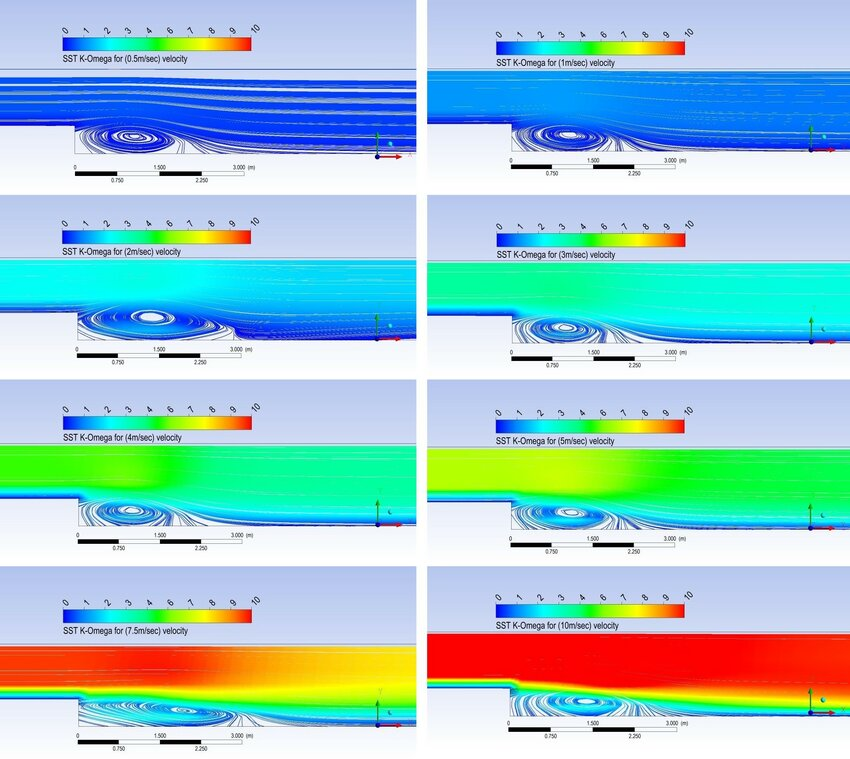
\includegraphics[width=0.8\textwidth]{figures/elocity-contour-for-different-values-of-velocity-for-SST-K-o-model.jpg.png}
    \caption{Figure for Comparison of k-epsilon vs. k-omega models.}
    \label{fig:k_epsilon_omega}
\end{figure}

\subsection{The SST (Shear Stress Transport) $k-\omega$ Model (Why it is chosen for Wall Heat Flux)}
\textit{Paper}
\par
To overcome the limitations of the standard two-equation models, Menter (1994) developed the Shear Stress Transport (SST) $k-\omega$ model. This model effectively blends the robust and accurate formulation of the $k-\omega$ model in the near-wall region with the freestream independence of the $k-\epsilon$ model in the far field.



\subsubsection*{1. Zonal Blending Functions}
The core innovation of the SST model is the use of a blending function, $F_1$, which transitions the model formulation based on the distance from the wall ($y$).
\begin{itemize}
    \item \textbf{Near Wall ($F_1 = 1$):} The model activates the standard $k-\omega$ equations, allowing for direct resolution of the viscous sublayer without damping functions. This ensures accurate prediction of wall heat flux ($q_w$) and wall shear stress ($\tau_w$).
    \item \textbf{Far Field ($F_1 = 0$):} The model smoothly transitions to the $k-\epsilon$ formulation (mathematically transformed into $k-\omega$ variables). This eliminates the sensitivity to freestream turbulence properties that plagues the standard $k-\omega$ model.
\end{itemize}

\subsubsection*{2. The Shear Stress Limiter}
In flows with strong adverse pressure gradients—such as the deceleration zone in the valleys of a scalloped IAD—standard two-equation models often over-predict the eddy viscosity ($\mu_t$). This leads to a failure to predict flow separation, resulting in erroneous aerodynamic coefficients.

The SST formulation introduces a limiter to the eddy viscosity definition to satisfy the Bradshaw assumption (that shear stress is proportional to kinetic energy in boundary layers):

\begin{equation}
    \mu_t = \frac{\rho k}{\omega} \frac{1}{\max\left( \frac{1}{\alpha^*}, \frac{S F_2}{a_1 \omega} \right)}
\end{equation}

Where $S$ is the strain rate magnitude and $F_2$ is a second blending function. This limiter prevents the buildup of excessive turbulence levels in stagnation regions and separation zones.

\subsubsection*{Justification for HIAD Analysis}
For this research, the SST $k-\omega$ model is selected as the turbulence closure for the following reasons:
\begin{enumerate}
    \item \textbf{Heat Transfer Accuracy:} It is widely regarded as the industry standard for aerodynamic heating predictions \cite{menter1994SST}, typically predicting heat flux within 5-10\% of experimental data for attached flows.
    \item \textbf{Separation Prediction:} The shear stress transport formulation is critical for accurately capturing the size and stability of the recirculation vortices inside the toroidal valleys, which directly drive the local thermal environment.
\end{enumerate}

\section{Thermodynamic Gas Models}

\par
In standard aerodynamic analysis (subsonic or supersonic), air is typically modeled as a Calorically Perfect Gas. This assumes that the specific heats ($C_p$ and $C_v$) are constant and that the internal energy is a linear function of temperature ($e = C_v T$). However, for a vehicle entering the atmosphere at hypersonic speeds ($Ma > 5$), this assumption breaks down catastrophicallly \cite{AndersonHypersonic}.
\par
The immense kinetic energy converted into heat across the bow shock raises the gas temperature to levels where the internal structure of the air molecules is altered. As the temperature rises, the gas undergoes a sequence of energy mode excitations:
\begin{itemize}
    \item \textbf{$T > 800$ K:} Vibrational excitation of $N_2$ and $O_2$ molecules becomes significant. The gas becomes Thermally Perfect but Calorically Imperfect ($C_p = f(T)$).
    \item \textbf{$T > 2000$ K:} Oxygen molecules begin to dissociate ($O_2 \rightarrow 2O$).
    \item \textbf{$T > 4000$ K:} Nitrogen molecules begin to dissociate ($N_2 \rightarrow 2N$).
    \item \textbf{$T > 9000$ K:} Atoms begin to ionize ($N \rightarrow N^+ + e^-$).
\end{itemize}

Accurately modeling these phenomena is essential for an Inflatable Aerodynamic Decelerator (IAD). Failure to account for variable specific heat, for instance, can lead to an over-prediction of the post-shock temperature and a significant under-prediction of the density, resulting in incorrect shock stand-off distances and non-physical heat flux results.


\subsection{The Equation of State: Ideal Gas vs. Real Gas Effects}

\par
The Equation of State relates the thermodynamic properties of pressure ($p$), density ($\rho$), and temperature ($T$). In standard aerodynamic analysis, the air is treated as an Ideal Gas, obeying the relation:

\begin{equation}
    p = \rho R T
\end{equation}

Where $R$ is the specific gas constant ($R = 287$ J/kg$\cdot$K for air). This relation assumes that intermolecular forces are negligible and the volume of the molecules themselves is zero \cite{AndersonHypersonic}.



In the context of hypersonic re-entry, the term "Real Gas Effects" is often used broadly to describe deviations from standard air behavior. However, it is important to distinguish between two types of deviations:

\begin{enumerate}
    \item \textbf{Dense Gas Effects (Intermolecular Forces):} At extremely high pressures (e.g., deep atmospheric entry on Gas Giants), gas molecules are packed so tightly that intermolecular forces become significant. In this regime, the Ideal Gas Law is invalid, and a compressibility factor $Z$ is introduced ($p = \rho Z R T$). For Earth re-entry at high altitudes (low density), these effects are typically negligible, and the Ideal Gas EOS ($p = \rho R T$) remains valid.
    
    \item \textbf{High-Temperature Effects (Chemistry):} This is the dominant "Real Gas" effect for HIADs. As temperature increases, the chemical composition of the air changes (dissociation). While the equation $p = \rho R_{mix} T$ still holds, the gas constant $R_{mix}$ is no longer constant because the molecular weight of the mixture changes as $N_2$ and $O_2$ break apart.
\end{enumerate}

A comparison of these modeling assumptions is presented in Table \ref{tab:gas_models}.

\begin{table}[H]
    \centering
    \caption{Comparison of Gas Models in Hypersonic Aerodynamics.}
    \label{tab:gas_models}
    \begin{tabularx}{\textwidth}{|l|X|X|}
        \hline
        \rowcolor{gray!20} \textbf{Feature} & \textbf{Ideal (Perfect) Gas Model} & \textbf{Real Gas (Hypersonic) Model} \\ \hline
        \textbf{Equation of State} & $p = \rho R T$ (Constant $R$) & $p = \rho R_{mix} T$ (Variable $R$ due to chemistry) \\ \hline
        \textbf{Specific Heats} & Constant ($C_p, C_v = \text{const}$) & Variable ($C_p(T)$) due to vibrational excitation. \\ \hline
        \textbf{Internal Energy} & $e = C_v T$ (Linear) & $e = f(T)$ (Non-linear, includes chemical potential). \\ \hline
        \textbf{Shock Density Ratio} & Limited to $(\gamma+1)/(\gamma-1) = 6$ & Can exceed 10 or 12 (Thinner shock layers). \\ \hline
        \textbf{Temperature Prediction} & Over-predicts post-shock temperature. & Lower temperature (Energy absorbed by chemistry). \\ \hline
    \end{tabularx}
\end{table}

\subsection{Calorically Perfect vs. Thermally Perfect Gas (Variable $C_p$)}

\par
The distinction between a calorically perfect and a thermally perfect gas lies in the behavior of the specific heat capacities ($C_p$ and $C_v$) as the temperature of the fluid increases.



\subsubsection*{1. Calorically Perfect Gas (CPG)}
At low temperatures (typically $T < 800$ K), the vibrational energy modes of the nitrogen and oxygen molecules are "frozen." The internal energy of the gas consists only of translational and rotational kinetic energy, which are fully excited at room temperature. Consequently, the specific heat at constant pressure ($C_p$) is constant, and the internal energy ($e$) is a linear function of temperature:
\begin{equation}
    e = C_v T \quad \text{and} \quad h = C_p T
\end{equation}
This assumption is valid for subsonic and low-supersonic flows but leads to significant errors in the hypersonic regime.
\par
\subsubsection*{2. Thermally Perfect Gas (TPG)}
As the gas temperature rises across a strong bow shock ($T > 800$ K), the collisions between molecules become energetic enough to activate the vibrational modes of the diatomic molecules ($N_2$ and $O_2$). These vibrational modes absorb a portion of the flow's kinetic energy, acting as an additional "heat sink."
\par
Mathematically, this means that the specific heats become functions of temperature:
\begin{equation}
    C_p = f(T) \quad \text{and} \quad C_v = f(T)
\end{equation}
However, the gas still obeys the thermal equation of state $p = \rho R T$ (assuming no chemical dissociation). A gas that satisfies $p=\rho R T$ but has variable specific heats is defined as a Thermally Perfect Gas.
\par
In CFD simulations for hypersonic re-entry, $C_p(T)$ is typically modeled using a polynomial curve fit, such as the NASA 7-coefficient or 9-coefficient polynomials:
\begin{equation}
    \frac{C_p(T)}{R} = a_1 + a_2 T + a_3 T^2 + a_4 T^3 + a_5 T^4
\end{equation}
Using a Thermally Perfect Gas model is essential for the HIAD analysis because the absorption of energy into vibrational modes lowers the peak shock layer temperature compared to a Calorically Perfect prediction, resulting in more accurate (and often less conservative) density and heat flux calculations \cite{AndersonHypersonic}.

\subsection{Temperature-Dependent Viscosity (Sutherland’s Law)}

In classical low-speed aerodynamics, fluid viscosity is often treated as a constant property. However, in the hypersonic regime where temperature variations within the shock layer can span thousands of degrees, the viscosity of the gas changes largely. Unlike liquids, where viscosity decreases with heat, the viscosity of a gas \textit{increases} with temperature due to the increased molecular agitation and momentum exchange between fluid layers.
\par
To accurately model the viscous stresses and heat transfer in the boundary layer, the dynamic viscosity ($\mu$) must be coupled to the local static temperature ($T$). The standard model used in compressible flow CFD is Sutherland’s Law (1893), which is derived from the kinetic theory of gases using an idealized intermolecular potential \cite{AndersonHypersonic}.

\begin{equation}
    \mu(T) = \mu_{ref} \left( \frac{T}{T_{ref}} \right)^{3/2} \frac{T_{ref} + S}{T + S}
\end{equation}

Where:
\begin{itemize}
    \item $\mu$ is the dynamic viscosity at temperature $T$.
    \item $\mu_{ref}$ is the reference viscosity at reference temperature $T_{ref}$.
    \item $S$ is the Sutherland constant (effective temperature), which accounts for intermolecular attraction.
\end{itemize}

For standard air, the coefficients used in this study are:
\begin{itemize}
    \item $\mu_{ref} = 1.716 \times 10^{-5}$ kg/(m$\cdot$s)
    \item $T_{ref} = 273.15$ K
    \item $S = 110.4$ K
\end{itemize}

Implementing Sutherland's Law is vital for the thermal analysis of an IAD. Since aerodynamic heating is directly proportional to the square root of the viscosity product ($q_w \propto \sqrt{\rho \mu}$), neglecting the temperature dependence of $\mu$ would result in a gross underestimation of the surface heat flux.

\begin{figure}[H]
    \centering
    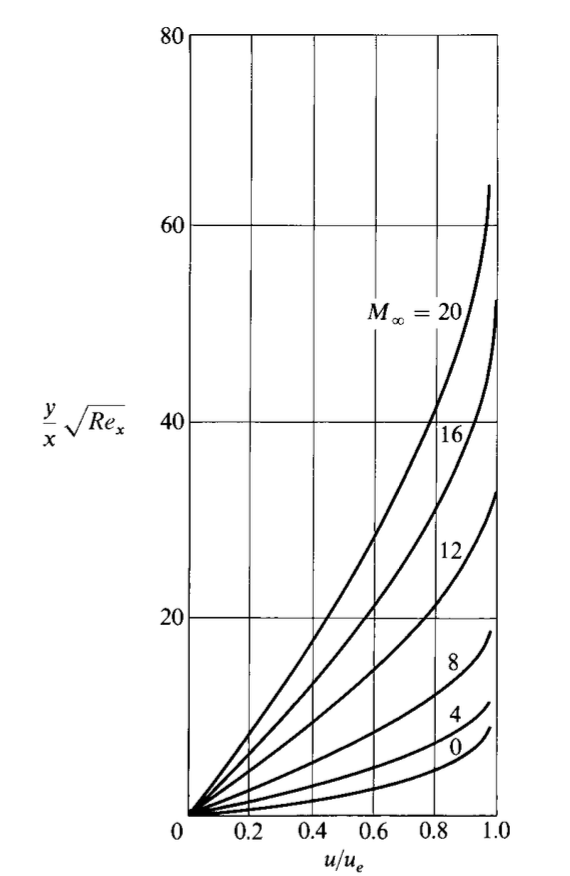
\includegraphics[width=0.4\textwidth]{figures/sutherlandfx.png}
    \caption{(Sutherland’s Law effect on Laminar Boundary Layer Insulated Flat Plate).}
    \label{fig:sutherlands_law}
\end{figure}

\section{Numerical Solvers and Schemes}
The numerical simulation of hypersonic flow fields requires a solver architecture capable of handling the strong coupling between the velocity field, density, and energy equation. For this study, the Density-Based Coupled Solver is selected over the traditional Pressure-Based solver \cite{versteeg2007cfd}.

\subsection{Density-Based Solver Formulation}
In low-speed (incompressible) flows, density is constant, and the pressure field is derived from the continuity equation (typically using algorithms like SIMPLE or PISO). However, in hypersonic flows ($Ma > 5$), density is a variable function of pressure and temperature (via the Equation of State).

The Density-Based solver integrates the continuity, momentum, energy, and species transport equations simultaneously (coupled) rather than sequentially.
\begin{itemize}
    \item \textbf{Coupling:} The governing equations are solved as a vector system. This robust coupling is essential for resolving the high-gradient shock structures where density changes abruptly.
    \item \textbf{Time Formulation:} An Implicit formulation is employed to allow for larger Courant-Friedrichs-Lewy (CFL) numbers while maintaining unconditional stability during the convergence process towards a steady-state solution.
\end{itemize}


\subsection{Flux Discretization Schemes}
To compute the fluxes of mass, momentum, and energy across the cell faces, specific discretization schemes are chosen to balance numerical stability with accuracy.

\subsubsection*{1. Convective Flux Type: Roe-FDS}
The Roe Flux-Difference Splitting (Roe-FDS) scheme is selected for the inviscid flux formulation. The Roe scheme is a Godunov-type upwind method that solves an approximate Riemann problem at each cell face.
\begin{itemize}
    \item \textbf{Justification:} It is widely renowned for its superior shock-capturing capabilities, providing crisp resolution of discontinuities (shocks) without introducing excessive numerical diffusion (smearing) \cite{versteeg2007cfd}.
\end{itemize}

\subsubsection*{2. Spatial Discretization: Second-Order Upwind}
To ensure the solution is grid-independent and physically accurate:
\begin{itemize}
    \item \textbf{Gradients:} The Least Squares Cell-Based method is used to compute gradients, as it is less sensitive to grid skewness on the unstructured mesh of the scalloped toroids.
    \item \textbf{Flow Variables:} A Second-Order Upwind scheme is applied to the flow, turbulence, and energy equations. This scheme reconstructs face values using a Taylor series expansion from the cell center, offering significantly higher accuracy than First-Order schemes, which are prone to false diffusion that can artificially thicken the bow shock.
\end{itemize}


\subsection{Shock Capturing Schemes (Upwind, Flux splitting)}
The defining characteristic of hypersonic flow is the presence of strong discontinuities (shock waves) where flow properties change abruptly over a microscopic distance. Standard central-difference schemes, commonly used in subsonic flow, are non-dissipative and essentially "blind" to the direction of flow propagation. When applied to a shock wave, they invariably produce unphysical oscillations (Gibbs phenomenon) that lead to solution divergence.

To resolve these discontinuities without numerical instability, modern CFD relies on Shock Capturing techniques rooted in the mathematical theory of hyperbolic conservation laws \cite{versteeg2007cfd}.



\subsubsection{The Upwind Philosophy}
The physical basis for upwinding is the transport of information. In supersonic flow, disturbances cannot propagate upstream against the flow; information travels only along characteristic lines from upstream to downstream.
\begin{itemize}
    \item \textbf{Concept:} The numerical flux at a cell face should be calculated using the state variables from the "upwind" side (the side from which the fluid is flowing).
    \item \textbf{Implementation:} First-order upwind schemes simply take the cell center value of the upstream cell. While stable, this is highly diffusive, causing sharp shock waves to appear "smeared" across many grid cells.
    \item \textbf{High-Resolution Schemes:} To achieve accuracy, Second-Order Upwind schemes are employed. These reconstruct the face value using a Taylor series expansion based on upstream gradients. To prevent oscillations near shocks, Flux Limiters (e.g., Min-Mod, Barth-Jespersen) are applied to strictly enforce monotonicity (TVD - Total Variation Diminishing properties).
\end{itemize}

\subsubsection{Flux Splitting Schemes}
To mathematically determine "which way is upstream" for the complex system of Navier-Stokes equations (where sound waves can travel in multiple directions), Flux Splitting methods are used. These schemes decompose the total flux into wave components.

\textbf{1. Flux Vector Splitting (FVS):}
Methods like \textit{Steger-Warming} or \textit{Van Leer} split the flux vector into positive (forward-moving) and negative (backward-moving) components based on the sign of the eigenvalues (wave speeds).
\begin{equation}
    F = F^+(\lambda^+) + F^-(\lambda^-)
\end{equation}
While robust, FVS schemes are known to be excessively dissipative in boundary layers, often over-predicting skin friction and heat transfer.

\textbf{2. Flux Difference Splitting (FDS) - The Preferred Choice:}
Methods like Roe’s Scheme (Approximate Riemann Solver) model the interface between two cells as a localized shock tube problem (Riemann problem).
\begin{itemize}
    \item Instead of splitting the flux itself, Roe's scheme solves for the difference in flux across the wave structure.
    \item \textbf{Relevance to HIADs:} FDS schemes are significantly less dissipative than FVS schemes. This makes them the standard choice for hypersonic viscous flows because they can accurately capture the crispness of the bow shock while simultaneously resolving the delicate shear gradients in the boundary layer \cite{toro2009riemann}.
\end{itemize}

\textbf{3. AUSM (Advection Upstream Splitting Method):}
A hybrid approach often used in modern codes (like ANSYS Fluent's "AUSM+" option). It splits the flux into a convective term (treated as a scalar) and a pressure term (treated acoustically). This method is designed to be as accurate as Roe's scheme but more robust against the "carbuncle phenomenon" (a numerical instability often seen near the stagnation point of blunt bodies).s
